\documentclass[12pt,a4paper]{article}

\usepackage[utf8]{inputenc}
\usepackage{graphicx}
\usepackage{hyperref}
\usepackage{booktabs}
\usepackage{amsmath}
\usepackage{amssymb}
\usepackage{listings}
\usepackage{xcolor}
\usepackage{titlesec}
\usepackage{float}
\usepackage{caption}

\hypersetup{
    colorlinks=true,
    linkcolor=black,
    filecolor=black,
    urlcolor=black,
}

\titleformat*{\section}{\LARGE\bfseries}
\titleformat*{\subsection}{\large\bfseries}
\titleformat*{\subsubsection}{\normalsize\bfseries\itshape}

\titlespacing\section{0pt}{12pt}{6pt}
\titlespacing\subsection{0pt}{10pt}{4pt}
\titlespacing\subsection{0pt}{8pt}{3pt}

\definecolor{codegreen}{rgb}{0,0.6,0}
\definecolor{codegray}{rgb}{0.5,0.5,0.5}
\definecolor{codepurple}{rgb}{0.58,0,0.82}
\definecolor{backcolour}{rgb}{0.95,0.95,0.92}

\lstdefinestyle{pystyle}{
    backgroundcolor=\color{backcolour},
    commentstyle=\color{codegreen},
    keywordstyle=\color{blue},
    numberstyle=\tiny\color{codegray},
    stringstyle=\color{codepurple},
    basicstyle=\ttfamily\scriptsize,
    breaklines=true,
    frame=single,
    numbers=left,
    xleftmargin=5mm,
    xrightmargin=5mm
}

\lstdefinestyle{jsonstyle}{
    backgroundcolor=\color{backcolour},
    commentstyle=\color{codegreen},
    numberstyle=\tiny\color{codegray},
    basicstyle=\ttfamily\scriptsize,
    breaklines=true,
    frame=single,
    numbers=left,
    xleftmargin=5mm,
    xrightmargin=5mm
}

\lstdefinestyle{javascriptstyle}{
    backgroundcolor=\color{backcolour},
    commentstyle=\color{codegreen},
    keywordstyle=\color{blue},
    numberstyle=\tiny\color{codegray},
    stringstyle=\color{codepurple},
    basicstyle=\ttfamily\scriptsize,
    breaklines=true,
    frame=single,
    numbers=left,
    xleftmargin=5mm,
    xrightmargin=5mm
}

\lstset{
    breaklines=true,
    postbreak=\space,
    defaultdialect=Python
}

\usepackage[a4paper,margin=1in]{geometry}
\usepackage{tikz}
\usepackage{eso-pic}
\usetikzlibrary{calc}

% \AddToShipoutPictureBG{%
%   \begin{tikzpicture}[remember picture,overlay]
%     \draw[thick]
%       ([xshift=0.3in,yshift=0.3in]current page.south west)
%       rectangle
%       ([xshift=-0.3in,yshift=-0.3in]current page.north east);
%   \end{tikzpicture}
% }

\usepackage{fancyhdr}

\begin{document}
% Table of Contents - roman page numbers
\pagenumbering{roman}
\tableofcontents

\clearpage

\pagestyle{fancy}
\fancyhf{} % clear all default headers/footers

% ---------------------------------------------HEADER----------------------------------
\fancyhead[L]{Temporal Interview Profiling System (TIPS) - 2026}
% ---------------------------------------------FOOTER----------------------------------
\fancyfoot[L]{School of CSA, REVA University, Bengaluru}
\fancyfoot[R]{\thepage}

\renewcommand{\headrulewidth}{0.4pt}
\renewcommand{\footrulewidth}{0.4pt}
% -------------------------------------------END---------------------------------------

% Main content - arabic page numbers
\pagenumbering{arabic}

\section{Introduction}

\subsection{Background and Motivation}

In the modern recruitment landscape, technical interviews serve as a critical bottleneck in the hiring process. Organizations invest significant resources in conducting interviews, yet the evaluation process often remains subjective and inconsistent. Interviewers may have varying criteria, unconscious biases can influence decisions, and the sheer volume of candidates makes thorough manual analysis impractical.

Automated interview analysis systems have emerged as a promising solution to address these challenges. By leveraging advances in speech recognition, computer vision, natural language processing, and machine learning, these systems can extract meaningful signals from interview recordings that might otherwise go unnoticed during traditional evaluation methods.

The Temporal Interview Profiling System (TIPS) represents an attempt to build a comprehensive interview analysis pipeline that goes beyond simple keyword matching or sentiment analysis. TIPS is designed to capture the temporal dynamics of interviews—understanding not just what candidates say, but how their confidence evolves throughout the interview, when they demonstrate expertise or hesitation, and how their responses align with the specific requirements of the position.

A key design philosophy of TIPS is modularity. Rather than building a monolithic system that handles all aspects of interview analysis, TIPS implements a six-stage pipeline where each stage focuses on a specific aspect of the analysis. This modular approach allows for easier debugging, optimization, and future enhancement of individual components.

Furthermore, TIPS is designed to function as a backend service that can be integrated with existing interview platforms. The Interview UI component serves as a data collection mechanism, allowing organizations to attach TIPS to their existing infrastructure. This addon approach means that companies with established interview systems can leverage TIPS's analytical capabilities without replacing their entire technology stack.

The TIPS system consists of three primary components:

\begin{enumerate}
    \item \textbf{Interview Recording UI}: A WebRTC-based browser interface for recording video interviews with synchronized audio capture.
    \item \textbf{Backend Pipeline}: A six-stage processing system that analyzes recorded interviews and generates behavioral metrics and semantic relevance scores.
    \item \textbf{Dashboard}: An interactive web-based visualization interface for presenting and exploring analysis results.
\end{enumerate}

These three components work together to provide a complete end-to-end solution for automated interview analysis, from recording to final recommendation.

\subsection{Problem Statement}

Traditional interview evaluation methods suffer from several significant limitations:

\begin{enumerate}
    \item \textbf{Subjectivity}: Human interviewers bring inherent biases and varying evaluation standards that lead to inconsistent assessments.
    
    \item \textbf{Limited Analysis Depth}: Manual evaluation can only process a fraction of the available information in an interview recording. Vocal characteristics, response patterns, and temporal dynamics are often overlooked.
    
    \item \textbf{Scalability Issues}: As organizations grow, the time required for thorough interview evaluations increases linearly, creating bottlenecks in the hiring pipeline.
    
    \item \textbf{Lack of Standardization}: Without automated tools, comparing candidates across different interviewers or time periods becomes challenging.
    
    \item \textbf{No Temporal Insights}: Traditional scoring provides a single aggregate score without understanding how candidate performance evolves throughout the interview.
    
    \item \textbf{Manual Processing}: Interview recordings require manual review, which is time-consuming and prone to human error.
    
    \item \textbf{Inconsistent Recording}: Different interview platforms produce recordings in various formats, making centralized analysis difficult.
\end{enumerate}

TIPS addresses these problems by providing an automated, reproducible, and comprehensive analysis system that processes interview recordings to generate temporal behavioral metrics and semantic relevance scores. The integrated Interview Recording UI ensures consistent recording format, while the Dashboard provides intuitive visualization of analysis results.

\subsection{Objectives}

The primary objectives of the TIPS project are:

\begin{enumerate}
    \item To develop a multi-stage backend pipeline that processes recorded interview files through sequential and parallel processing stages.
    
    \item To extract and analyze audio signals including speech transcription, voice activity patterns, pitch, energy, and speech rate.
    
    \item To analyze video signals including facial presence, head pose, gaze stability, and expression changes.
    
    \item To perform temporal segmentation that accurately pairs interviewer questions with candidate answers.
    
    \item To compute behavioral metrics that indicate candidate confidence, fluency, and engagement.
    
    \item To implement LLM-based semantic relevance scoring that evaluates candidate responses against job descriptions.
    
    \item To generate time-evolving candidate scores with incremental verdict recommendations.
    
    \item To design and implement a Dashboard visualization system for presenting analysis results.
    
    \item To implement a WebRTC-based Interview Recording UI for capturing synchronized video interviews.
    
    \item To create a unified system that seamlessly integrates recording, processing, and visualization components.
\end{enumerate}

\subsection{Scope}

The scope of this project encompasses:

\begin{itemize}
    \item \textbf{Interview Recording UI}: Complete WebRTC-based recording interface for conducting video interviews.
    \item \textbf{Backend Pipeline}: Complete implementation of the six-stage processing pipeline.
    \item \textbf{Dashboard}: Complete implementation of the visualization interface with five main views.
    \item \textbf{Integration}: System designed to function as a complete end-to-end solution for interview analysis.
\end{itemize}

The system is designed for batch processing of pre-recorded interviews rather than real-time streaming analysis. This approach allows for more comprehensive processing at the cost of immediate feedback. The Interview Recording UI captures interviews and saves them in a standardized format, which is then processed by the backend pipeline.

\clearpage

% ============================================================================
% SECTION 2: LITERATURE SURVEY
% ============================================================================

\section{Literature Survey}

The development of TIPS draws upon several domains of research and existing systems. This section surveys relevant work in automated interview analysis, behavioral signal processing, and LLM-based evaluation systems.

\subsection{Automated Interview Systems}

Several commercial and academic systems have explored automated interview analysis. Platforms such as HireVue, Pymetrics, and Codility offer video-based interview assessments with varying levels of automation. These systems typically focus on specific aspects such as facial expression analysis, keyword detection, or game-based assessments.

Research in this area has explored various modalities for interview analysis:

\begin{itemize}
    \item \textbf{Vocal Analysis}: Studies have shown correlations between vocal features (pitch, speech rate, hesitation patterns) and personality traits and emotional states.
    
    \item \textbf{Facial Expression Analysis}: Computer vision techniques have been applied to detect emotions, engagement levels, and authenticity of responses.
    
    \item \textbf{Content Analysis}: Natural Language Processing (NLP) techniques analyze the semantic content of responses for relevance, coherence, and technical accuracy.
\end{itemize}

However, many existing systems treat these modalities in isolation or provide only aggregate scores without temporal context. TIPS aims to provide a more holistic analysis by combining multiple signals and tracking their evolution throughout the interview.

TIPS differentiates itself from existing solutions by:

\begin{itemize}
    \item Providing time-evolving scores that track candidate performance throughout the interview
    \item Combining behavioral metrics with semantic relevance scoring
    \item Offering an integrated recording solution through WebRTC
    \item Providing a comprehensive dashboard for result visualization
    \item Using lightweight LLM models that can run on consumer hardware
\end{itemize}

\subsection{Speech Recognition and Transcription}

The field of automatic speech recognition (ASR) has seen dramatic improvements in recent years, particularly with the advent of transformer-based models. Faster-Whisper, used in TIPS for transcription, represents the state-of-the-art in open-source speech recognition, offering high accuracy with efficient inference.

Key advances that enable systems like TIPS include:

\begin{itemize}
    \item End-to-end neural network architectures
    \item Word-level timestamps for precise temporal alignment
    \item Voice Activity Detection (VAD) for identifying speech segments
    \item Multilingual support and robust handling of various accents
\end{itemize}

TIPS leverages Faster-Whisper's capabilities to generate accurate transcriptions with word-level timestamps, enabling precise Q\&A pairing in the temporal segmentation stage.

\subsection{Behavioral Signal Processing}

Behavioral signal processing involves extracting meaningful indicators from raw audio and video data. In the context of interview analysis, relevant signals include:

\begin{itemize}
    \item \textbf{Prosodic Features}: Pitch (fundamental frequency), energy (loudness), and speech rate provide indicators of confidence and engagement.
    
    \item \textbf{Voice Quality}: Measures of jitter, shimmer, and harmonics-to-noise ratio indicate vocal strain or emotional state.
    
    \item \textbf{Facial Features}: Face detection, landmark tracking, and pose estimation provide information about candidate attention and engagement.
    
    \item \textbf{Gaze and Eye Contact}: Eye tracking and gaze stability analysis indicate comfort level and attention.
\end{itemize}

TIPS implements feature extraction at both the frame level (for video) and the segment level (for audio) to build a comprehensive behavioral profile.

\subsection{LLM-Based Evaluation}

The emergence of Large Language Models (LLMs) has opened new possibilities for semantic evaluation. Unlike traditional keyword matching approaches, LLMs can understand context, evaluate technical accuracy, and provide nuanced relevance assessments.

TIPS utilizes Qwen2.5-3B-Instruct, a quantized LLM that can run on consumer hardware, to:

\begin{itemize}
    \item Evaluate semantic relevance between candidate responses and job requirements
    \item Extract matched keywords from responses
    \item Assess competency dimensions (technical depth, system design, production experience, communication clarity, problem solving)
    \item Generate incremental verdicts throughout the interview
    \item Produce final hiring recommendations
\end{itemize}

The use of 4-bit quantization allows the model to run on GPUs with limited VRAM while maintaining reasonable accuracy.

\clearpage

% ============================================================================
% SECTION 3: SYSTEM ARCHITECTURE
% ============================================================================

\section{System Architecture}

This section presents the high-level architecture of TIPS, including the data flow diagram, processing model, and technology stack.

\subsection{High-Level Architecture}

TIPS follows a batch processing architecture where interview recordings are processed after the interview session concludes. The system consists of three primary components:

\begin{enumerate}
    \item \textbf{Interview UI Layer}: Browser-based recording interface using WebRTC for capturing synchronized video and audio.
    \item \textbf{Backend Pipeline}: Six-stage processing system for analysis
    \item \textbf{Dashboard}: Interactive visualization interface for results
\end{enumerate}

The data flow follows a unidirectional pipeline pattern: interviews are recorded through the Interview UI, raw media files are processed through successive pipeline stages, with each stage consuming the output of the previous stage and producing intermediate results.

\begin{figure}[htbp]
    \centering
    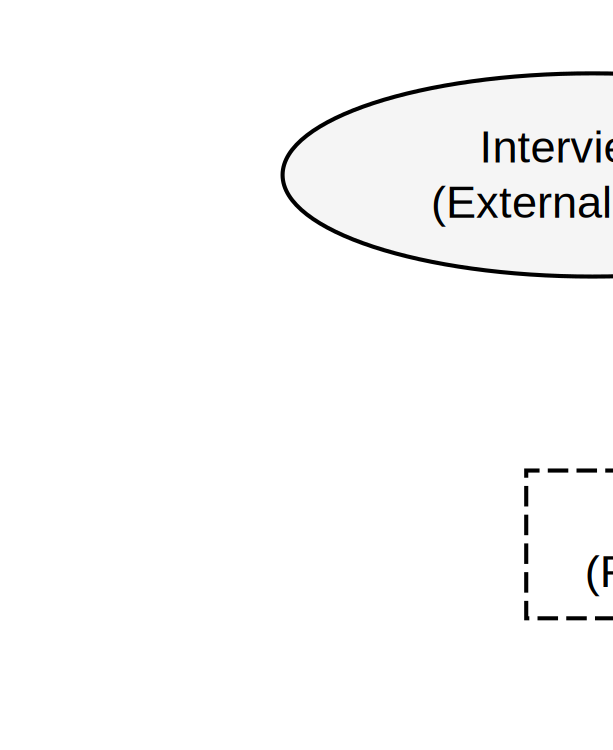
\includegraphics[width=1.1\textwidth]{tips_dfd.png}
    \caption{Data Flow Diagram of TIPS}
    \label{fig:dfd}
\end{figure}

Figure \ref{fig:dfd} illustrates the complete data flow from external entities (Interviewer and Candidate) through the various processing stages to the final output artifacts and Dashboard visualization.

The pipeline accepts four primary inputs:

\begin{itemize}
    \item \textbf{Interviewer Audio} (interviewer\_audio.wav): Recording of the interviewer's voice
    \item \textbf{Candidate Audio} (candidate\_audio.wav): Recording of the candidate's voice
    \item \textbf{Candidate Video} (candidate\_video.mp4): Recording of the candidate's video feed
    \item \textbf{Job Description}: Text document describing the position requirements
\end{itemize}

The output consists of JSON files containing timeline data, behavioral metrics, relevance scores, and candidate performance timelines. These outputs are consumed by the Dashboard for visualization.

The Interview Recording UI produces standardized output files in MP4 (video) and WAV (audio) formats, ensuring consistent input to the backend pipeline regardless of the recording platform used.

\subsection{Processing Model}

TIPS operates as a batch processing system rather than a real-time streaming system. This design choice reflects several considerations:

\begin{enumerate}
    \item \textbf{Comprehensive Analysis}: Batch processing allows for more thorough analysis since computational resources are not constrained by real-time requirements.
    
    \item \textbf{LLM Integration}: Large Language Models require the complete context (entire job description and full answers) for accurate evaluation, which is not compatible with streaming architectures.
    
    \item \textbf{Modularity}: Each stage can be independently optimized, debugged, or replaced without affecting others.
    
    \item \textbf{Scalability}: The pipeline can process multiple interviews concurrently without interference.
    
    \item \textbf{Post-Interview Review}: HR teams can review results after the interview is complete, allowing for more thoughtful evaluation.
\end{enumerate}

The processing flow consists of:

\begin{enumerate}
    \item \textbf{Sequential Stage 0}: Timebase establishment
    \item \textbf{Parallel Stages 1A, 1B, 1C}: Signal extraction (candidate audio, interviewer audio, candidate video)
    \item \textbf{Sequential Stage 2}: Temporal segmentation
    \item \textbf{Sequential Stage 3}: Behavioral metrics computation
    \item \textbf{Sequential Stage 4+5}: Semantic scoring and verdict aggregation
    \item \textbf{Dashboard Visualization}: Interactive exploration of results
\end{enumerate}

This hybrid approach maximizes parallelism where possible (Stage 1) while maintaining necessary sequential dependencies between stages.


\subsection{Stage 0: Timebase Establishment}

Stage 0 is the foundation of the entire pipeline. It establishes a canonical time base that synchronizes all subsequent processing stages. This stage extracts fundamental metadata from the input media files:

\begin{itemize}
    \item \textbf{Video Metadata}: Frame rate (FPS), total frame count, video duration
    \item \textbf{Audio Metadata}: Sample rate, channel count, audio duration
    \item \textbf{Timestamp Alignment}: Establishes the relationship between video frames and audio samples
    \item \textbf{Dataset Identification}: Assigns a unique identifier for tracking
\end{itemize}

This stage is critical because all subsequent stages rely on accurate timestamps. The timebase serves as the single source of truth for temporal calculations throughout the pipeline.

\subsection{Stages 1A, 1B, 1C: Parallel Signal Extraction}

Stage 1 represents the primary data extraction phase and is uniquely designed to maximize throughput through parallel processing. This stage consists of three independent sub-stages that execute simultaneously:

\begin{itemize}
    \item \textbf{Stage 1A - Candidate Audio Processing}: Processes the candidate's audio track to extract:
    \begin{itemize}
        \item Audio features (RMS energy, pitch) at regular intervals
        \item Voice Activity Detection (VAD) segments
        \item Speech transcription using Faster-Whisper
    \end{itemize}
    
    \item \textbf{Stage 1B - Interviewer Audio Processing}: Processes the interviewer's audio track to extract:
    \begin{itemize}
        \item Speech transcription for question identification
        \item Word-level timestamps for precise question boundaries
    \end{itemize}
    
    \item \textbf{Stage 1C - Candidate Video Processing}: Processes the candidate's video feed to extract:
    \begin{itemize}
        \item Sampled frames at regular intervals
        \item Face detection results
        \item Head pose estimation (yaw, pitch, roll)
        \item Gaze direction estimates
    \end{itemize}
\end{itemize}

The parallel execution of these three sub-stages significantly reduces overall processing time, as each operates on independent data sources.


\subsection{Stage 2: Temporal Segmentation}

Stage 2 combines the outputs from Stage 1 to create a unified temporal view of the interview. This stage performs two critical functions:

\begin{enumerate}
    \item \textbf{Speaking Segment Detection}: Identifies when each person (candidate and interviewer) is speaking based on voice activity segments from Stage 1A and transcription data from Stage 1B.
    
    \item \textbf{Q\&A Pairing}: Maps interviewer questions to candidate answers using a sophisticated algorithm:
    \begin{itemize}
        \item Questions are identified from interviewer transcription segments
        \item Candidate answers are matched to questions based on temporal proximity
        \item Silence within an answer window is tolerated (natural pauses)
        \item The next question marks the end of the current answer
    \end{itemize}
\end{enumerate}

The output of this stage provides the structural framework for all subsequent analysis.

\subsection{Stage 3: Behavioral Metrics Computation}

Stage 3 analyzes each candidate speaking segment in detail, computing quantitative metrics that indicate behavioral patterns:

\begin{itemize}
    \item \textbf{Audio Metrics}:
    \begin{itemize}
        \item Pitch (fundamental frequency) - indicates confidence and emotional state
        \item Energy (RMS) - indicates volume and assertiveness
        \item Speech rate - indicates fluency and preparation
        \item Pause density - indicates thinking time and hesitation
    \end{itemize}
    
    \item \textbf{Video Metrics}:
    \begin{itemize}
        \item Face presence ratio - indicates camera engagement
        \item Head motion - indicates nervousness or engagement
        \item Gaze stability - indicates eye contact quality
        \item Expression changes - indicates emotional engagement
    \end{itemize}
\end{itemize}

These metrics provide objective, quantifiable indicators of candidate performance that complement the semantic analysis in later stages.


\subsection{Stages 4 and 5: Semantic Scoring and Verdict Aggregation}

Stages 4 and 5 represent the intelligence layer of the TIPS pipeline, where Large Language Models (LLMs) evaluate the semantic content of candidate responses:

\begin{itemize}
    \item \textbf{Stage 4 - Semantic Relevance Scoring}:
    \begin{itemize}
        \item Evaluates each candidate answer against job description requirements
        \item Extracts matched keywords from technical vocabulary
        \item Assesses competency dimensions (technical depth, system design, production experience, communication clarity, problem solving)
        \item Generates incremental verdicts after each question
    \end{itemize}
    
    \item \textbf{Stage 5 - Verdict Aggregation}:
    \begin{itemize}
        \item Aggregates scores from all Q\&A pairs
        \item Computes final competency scores
        \item Generates hiring recommendation (STRONG\_HIRE, HIRE, BORDERLINE, NO\_HIRE)
        \item Provides confidence level and justification
    \end{itemize}
\end{itemize}

These stages utilize Qwen2.5-3B-Instruct with 4-bit quantization for efficient inference while maintaining evaluation quality.


\subsection{Technology Stack}

TIPS leverages a modern technology stack optimized for performance and accuracy:

\begin{table}[htbp]
    \centering
    \caption{Technology Stack - Backend Pipeline}
    \label{tab:tech_stack_backend}
    \begin{tabular}{@{}ll@{}}
        \toprule
        \textbf{Component} & \textbf{Technology} \\
        \midrule
        Programming Language & Python 3.11 \\
        Web Framework & FastAPI \\
        WebRTC & aiortc \\
        ASGI Server & uvicorn \\
        Speech-to-Text & faster-whisper (small model) \\
        Audio Analysis & librosa, webrtcvad \\
        Video Processing & OpenCV, MediaPipe \\
        LLM Inference & Transformers + PyTorch \\
        LLM Quantization & BitsAndBytes (4-bit NF4) \\
        Video Codec & ffmpeg, PyAV \\
        \bottomrule
    \end{tabular}
\end{table}

\begin{table}[htbp]
    \centering
    \caption{Technology Stack - Interview Recording UI}
    \label{tab:tech_stack_ui}
    \begin{tabular}{@{}ll@{}}
        \toprule
        \textbf{Component} & \textbf{Technology} \\
        \midrule
        Backend Server & FastAPI (Python) \\
        Real-time Communication & WebSocket \\
        Video/Audio Capture & WebRTC (Browser API) \\
        Media Processing & aiortc (Python) \\
        Video Codec & H.264 (browser + ffmpeg) \\
        Audio Codec & Opus (browser) \\
        Frontend & HTML5, CSS3, JavaScript (ES6+) \\
        \bottomrule
    \end{tabular}
\end{table}

\begin{table}[htbp]
    \centering
    \caption{Technology Stack - Dashboard}
    \label{tab:tech_stack_dashboard}
    \begin{tabular}{@{}ll@{}}
        \toprule
        \textbf{Component} & \textbf{Technology} \\
        \midrule
        Frontend Framework & Vanilla JavaScript (ES6 Modules) \\
        Routing & Custom SPA Router \\
        Data Visualization & Chart.js 4.4.2 \\
        Styling & CSS3 with Custom Properties \\
        Font & Inter, JetBrains Mono (Google Fonts) \\
        File Loading & Fetch API, File API \\
        Deployment & Static files (any web server) \\
        \bottomrule
    \end{tabular}
\end{table}

The LLM component uses Qwen2.5-3B-Instruct with 4-bit quantization, enabling operation on GPUs with limited VRAM (approximately 3GB) while maintaining reasonable inference quality.


\subsection{System Specifications}

The TIPS backend pipeline has been developed and tested on the following system configuration:

\begin{table}[htbp]
    \centering
    \caption{Development System Specifications}
    \label{tab:system_specs}
    \begin{tabular}{@{}ll@{}}
        \toprule
        \textbf{Component} & \textbf{Specification} \\
        \midrule
        Operating System & EndeavourOS (Arch Linux) x86\_64 \\
        Kernel & Linux 6.12.71-1-lts \\
        CPU & Intel Core i5-11300H @ 4.40 GHz (8 cores) \\
        GPU & NVIDIA GeForce RTX 3050 Mobile (4GB VRAM) \\
        Integrated GPU & Intel Iris Xe Graphics @ 1.30 GHz \\
        RAM & 23.26 GB DDR4 \\
        Display & 15.6" BOE0A81 @ 1920x1080, 120Hz \\
        Window Manager & i3 4.25.1 (X11) \\
        Terminal & tmux 3.6a \\
        Python Version & 3.11 \\
        \bottomrule
    \end{tabular}
\end{table}

The system leverages CUDA for GPU-accelerated LLM inference while using CPU-based processing for audio and video feature extraction where appropriate.

The development environment utilizes virtual environments for dependency isolation, with all required ML models pre-cached locally.

\clearpage

% ============================================================================
% PHASE 2: METHODOLOGY - BACKEND PIPELINE IMPLEMENTATION
% ============================================================================

\section{Methodology}

This section details the complete implementation of the TIPS backend pipeline. The pipeline consists of six stages, each designed to process specific aspects of the interview data. The pipeline follows a hybrid execution model where Stage 0 runs sequentially, Stages 1A/1B/1C run in parallel, and Stages 2-5 run sequentially.

The pipeline orchestration is handled by the main script \texttt{main.py}, which manages input preparation, stage execution, and output management.

\subsection{Pipeline Orchestration}

The main orchestration script handles backup of previous results, cleanup of temporary files, and result versioning.

The pipeline execution follows this workflow:

\begin{enumerate}
    \item \textbf{Input Preparation}: Symlinks are created in a temporary directory to reference the input files (video, audio files) and job description. This approach avoids copying large media files and allows for cleaner file management.
    
    \item \textbf{Stage 0 (Sequential)}: Timebase establishment - The pipeline first establishes a canonical time reference by extracting metadata from video and audio files, ensuring all subsequent stages use consistent timestamps.
    
    \item \textbf{Stages 1A, 1B, 1C (Parallel)}: Parallel signal extraction - Three independent processes extract raw signals from candidate audio, interviewer audio, and candidate video simultaneously, maximizing throughput.
    
    \item \textbf{Stage 2 (Sequential)}: Temporal segmentation - With all signals extracted, the system combines them to identify speaking segments and pair questions with answers.
    
    \item \textbf{Stage 3 (Sequential)}: Behavioral metrics computation - Each candidate speaking segment is analyzed to compute audio and video behavioral metrics.
    
    \item \textbf{Stage 4+5 (Sequential)}: Semantic scoring and verdict aggregation - The LLM processes each Q\&A pair to evaluate semantic relevance and generate incremental verdicts.
    
    \item \textbf{Output Generation}: All intermediate and final results are saved as JSON files with proper versioning for traceability.
\end{enumerate}

The orchestration script also handles error recovery, logging, and progress reporting. Each stage produces intermediate outputs that serve as inputs to subsequent stages, ensuring the pipeline can resume from a failed stage without reprocessing completed stages.


% ============================================================================
% SUBSECTION 4.1: STAGE 0 - TIMEBASE
% ============================================================================

\subsection{Stage 0: Timebase Establishment}

The first stage establishes a canonical time base for the entire pipeline by extracting timing metadata from the input media files.

\textbf{Objectives:}
\begin{itemize}
    \item Extract video frame rate and total frame count
    \item Calculate video duration
    \item Extract audio duration and sample rate
    \item Establish alignment between video and audio streams
\end{itemize}

\textbf{Implementation:}

The timebase stage uses OpenCV for video metadata extraction and librosa for audio metadata:

\begin{lstlisting}[style=pystyle]
def get_video_info(video_path):
    cap = cv2.VideoCapture(video_path)
    fps = cap.get(cv2.CAP_PROP_FPS)
    frame_count = int(cap.get(cv2.CAP_PROP_FRAME_COUNT))
    duration = frame_count / fps if fps > 0 else 0
    cap.release()
    return {"fps": fps, "frame_count": frame_count, "duration_sec": round(duration, 3)}

def get_audio_info(audio_path):
    info = librosa.info(audio_path)
    return {"duration_sec": round(info.get('duration', 0), 3), 
            "sample_rate": info.get('sr', 0)}
\end{lstlisting}

\textbf{Output:}

Stage 0 produces \texttt{timeline.json} containing:

\begin{lstlisting}[style=jsonstyle]
{
  "timebase": "video",
  "dataset_id": "1",
  "video": {
    "file": "path/to/video.mp4",
    "fps": 24.0,
    "frame_count": 9248,
    "duration_sec": 385.333
  },
  "audio": {
    "candidate": {"duration_sec": 385.333, "sample_rate": 48000},
    "interviewer": {"duration_sec": 385.333, "sample_rate": 48000}
  },
  "alignment": {"video_to_audio_offset_sec": 0.0}
}
\end{lstlisting}

This timeline serves as the reference for all subsequent stages, ensuring temporal alignment across different media streams.

\textbf{Technical Details:}

The timebase stage performs the following operations:

\begin{enumerate}
    \item \textbf{Video Metadata Extraction}: Uses OpenCV's VideoCapture to retrieve FPS, frame count, and duration. The FPS is critical for converting between frame indices and timestamps.
    
    \item \textbf{Audio Metadata Extraction}: Uses Librosa's info function to retrieve audio duration and sample rate. Falls back to soundfile if Librosa fails.
    
    \item \textbf{Alignment Calculation}: Computes the offset between video and audio streams. In typical interview recordings, the video and audio are synchronized at the start (offset = 0.0).
    
    \item \textbf{Dataset Identification}: Extracts dataset ID from the input filename for traceability.
\end{enumerate}

The timeline JSON serves as the master reference for all subsequent processing stages, ensuring that timestamps from different stages can be correctly correlated.


% ============================================================================
% SUBSECTION 4.2: STAGE 1 - SIGNAL EXTRACTION
% ============================================================================

\subsection{Stage 1: Signal Extraction}

Stage 1 consists of three parallel sub-stages that extract raw signals from the media files:

\begin{itemize}
    \item \textbf{Stage 1A}: Candidate Audio Processing
    \item \textbf{Stage 1B}: Interviewer Audio Processing  
    \item \textbf{Stage 1C}: Candidate Video Processing
\end{itemize}

These stages run in parallel to maximize throughput since they operate on independent data sources.

% ============================================================================
% SUBSECTION 4.2.1: STAGE 1A - CANDIDATE AUDIO
% ============================================================================

\subsection{Stage 1A: Candidate Audio Processing}

The candidate audio processing stage extracts low-level audio features, performs voice activity detection, and generates speech transcription.

\textbf{Components:}

\begin{enumerate}
    \item \textbf{Audio Feature Extraction}: Extracts RMS energy and pitch (fundamental frequency) at regular intervals.
    
    \item \textbf{Voice Activity Detection (VAD)}: Uses WebRTC VAD to identify speech segments.
    
    \item \textbf{Speech Transcription}: Uses Faster-Whisper for speech-to-text conversion with word-level timestamps.
\end{enumerate}

\textbf{Feature Extraction:}

\begin{lstlisting}[style=pystyle]
def extract_features(audio_path, sample_rate=16000):
    y, sr = librosa.load(audio_path, sr=sample_rate)
    frame_length = int(0.025 * sample_rate)
    hop_length = int(0.010 * sample_rate)
    
    rms = librosa.feature.rms(y=y, frame_length=frame_length, hop_length=hop_length)[0]
    pitches, magnitudes = librosa.piptrack(y=y, sr=sr, hop_length=hop_length)
    
    for i in range(0, len(rms), 10):
        timestamp = i * hop_length / sample_rate
        pitch_values = pitches[:, i]
        pitch = pitch_values[pitch_values > 0].mean() if np.any(pitch_values > 0) else 0
        
        features.append({
            "timestamp_sec": round(timestamp, 3),
            "rms_energy": round(float(rms[i]), 4),
            "pitch_hz": round(float(pitch), 2)
        })
    return features
\end{lstlisting}

\textbf{Speech Transcription:}

The system uses Faster-Whisper with the small model size for efficient inference:

\begin{lstlisting}[style=pystyle]
def transcribe(audio_path):
    model = WhisperModel("small", device="cpu", compute_type="int8")
    segments, info = model.transcribe(
        audio_path,
        word_timestamps=True,
        vad_filter=True,
        vad_parameters=dict(min_silence_duration_ms=700, speech_pad_ms=200)
    )
    return {"language": info.language, "segments": segments}
\end{lstlisting}

\textbf{Output:}

Stage 1A produces \texttt{candidate\_audio\_raw.json} containing:
\begin{itemize}
    \item Audio features (RMS energy, pitch) at 10-frame intervals
    \item Voice activity segments with start/end timestamps
    \item Transcription segments with word-level timestamps
\end{itemize}

Typical output includes approximately 3,800+ feature frames and 40-50 transcription segments per interview.

\textbf{Key Technologies:}

\begin{itemize}
    \item \textbf{Faster-Whisper}: An optimized implementation of Whisper that uses CTranslate2 for faster inference. The small model provides good balance between accuracy and speed.
    
    \item \textbf{WebRTC VAD}: Voice Activity Detection library that identifies speech segments in the audio stream. Uses aggressive mode (level 2) for better precision.
    
    \item \textbf{Librosa}: Used for audio feature extraction including RMS energy and pitch (fundamental frequency) computation.
\end{itemize}

The combination of VAD and Whisper's built-in voice activity detection provides robust speech segmentation, handling various speaking styles and pause patterns.


% ============================================================================
% SUBSECTION 4.2.2: STAGE 1B - INTERVIEWER AUDIO
% ============================================================================

\subsection{Stage 1B: Interviewer Audio Processing}

The interviewer audio processing stage focuses solely on speech transcription, as behavioral analysis is not needed for the interviewer's voice.

\textbf{Implementation:}

\begin{itemize}
    \item Uses Faster-Whisper for speech-to-text conversion
    \item Generates word-level timestamps for question identification
    \item Produces interview segments with timing information
\end{itemize}

\textbf{Output:}

Stage 1B produces \texttt{interviewer\_transcript.json} containing:
\begin{itemize}
    \item Transcribed segments with start/end timestamps
    \item Word-level timestamps for precise question boundaries
    \item Language detection and confidence scores
\end{itemize}

This transcription is crucial for Stage 2 (Temporal Segmentation) as it provides the question boundaries needed to pair questions with answers.

\textbf{Processing Details:}

The interviewer transcription differs from candidate audio processing in several ways:

\begin{enumerate}
    \item \textbf{No Feature Extraction}: Interviewer audio features (pitch, energy) are not computed as behavioral analysis focuses on the candidate.
    
    \item \textbf{Question Identification}: Word-level timestamps allow precise identification of when questions start and end.
    
    \item \textbf{Silence Handling}: Gaps between interviewer utterances are preserved to identify natural question boundaries.
    
    \item \textbf{Language Detection}: Automatic language detection ensures transcription accuracy.
\end{enumerate}

The output is used to segment the interview into Q\&A pairs, making it a critical input for the temporal segmentation stage.

% ============================================================================
% SUBSECTION 4.2.3: STAGE 1C - CANDIDATE VIDEO
% ============================================================================


\subsection{Stage 1C: Candidate Video Processing}

The candidate video processing stage extracts visual features from the recorded video, sampling frames at regular intervals for efficiency.

\textbf{Processing Steps:}

\begin{enumerate}
    \item \textbf{Frame Sampling}: Every 10th frame is sampled to reduce processing load while maintaining temporal resolution.
    
    \item \textbf{Face Detection}: Uses Haar Cascade classifiers to detect faces in each frame.
    
    \item \textbf{Head Pose Estimation}: Estimates yaw, pitch, and roll angles of the head.
    
    \item \textbf{Gaze Estimation}: Analyzes eye positions to estimate gaze direction.
\end{enumerate}

\textbf{Implementation:}

\begin{lstlisting}[style=pystyle]
def process_video(video_path, timeline):
    fps = timeline["video"]["fps"]
    frame_interval = int(fps / 10)  # Sample every 10th frame
    
    cap = cv2.VideoCapture(video_path)
    frame_idx = 0
    while cap.isOpened():
        ret, frame = cap.read()
        if not ret: break
        
        if frame_idx % frame_interval == 0:
            timestamp = frame_idx / fps
            
            # Face detection
            gray = cv2.cvtColor(frame, cv2.COLOR_BGR2GRAY)
            faces = face_cascade.detectMultiScale(gray, 1.3, 5)
            
            # Feature extraction for each detected face
            for (x, y, w, h) in faces:
                # Extract landmarks and compute pose
                landmarks = face_landmarker.compute_face_landmarks(frame)
                
        frame_idx += 1
    cap.release()
\end{lstlisting}

\textbf{Output:}

Stage 1C produces \texttt{candidate\_video\_raw.json} containing:
\begin{itemize}
    \item Sampled frames with timestamps (typically 900+ frames per interview)
    \item Face detection results (bounding boxes, confidence)
    \item Head pose angles (yaw, pitch, roll)
    \item Gaze direction estimates
    \item Face presence ratio
\end{itemize}

This data forms the basis for behavioral analysis in Stage 3.

\textbf{Video Processing Pipeline:}

The video processing stage implements a sophisticated feature extraction pipeline:

\begin{enumerate}
    \item \textbf{Frame Decoding}: Video frames are decoded using OpenCV's VideoCapture. Every Nth frame is sampled based on the target processing rate.
    
    \item \textbf{Color Space Conversion}: Frames are converted from BGR to grayscale for face detection, while color frames are preserved for expression analysis.
    
    \item \textbf{Face Detection}: Haar Cascade classifiers provide fast face detection. For each detected face, bounding box coordinates are recorded.
    
    \item \textbf{Facial Landmark Detection}: MediaPipe face mesh provides 468 landmarks for precise facial feature tracking.
    
    \item \textbf{Pose Estimation}: Head orientation is estimated from facial landmarks, providing yaw (left-right), pitch (up-down), and roll (tilt) angles.
    
    \item \textbf{Gaze Analysis}: Eye landmark positions are used to estimate gaze direction, indicating whether the candidate is looking at the camera, screen, or elsewhere.
\end{enumerate}

The sampling strategy (every 10th frame) provides approximately 24-30 frames per second of video, balancing computational efficiency with temporal resolution.


% ============================================================================
% SUBSECTION 4.3: STAGE 2 - TEMPORAL SEGMENTATION
% ============================================================================

\subsection{Stage 2: Temporal Segmentation}

Stage 2 combines the outputs from Stage 1 to create a unified temporal view of the interview, identifying speaking segments and pairing questions with answers.

\textbf{Objectives:}
\begin{itemize}
    \item Identify all speaking segments (candidate and interviewer)
    \item Detect silence intervals
    \item Map interviewer questions to candidate answers (Q\&A pairing)
\end{itemize}

\textbf{Speaking Segment Detection:}

The system uses voice activity detection from Stage 1A to identify when the candidate is speaking. Each segment is labeled as either "speaking" or "non-speaking":

\begin{lstlisting}[style=jsonstyle]
{
  "segment_id": "SEG1",
  "start_time": 1.65,
  "end_time": 1.83,
  "type": "speaking"
}
\end{lstlisting}

\textbf{Q\&A Pairing Algorithm:}

The pairing algorithm follows a SET-BASED approach:

\begin{enumerate}
    \item All candidate speaking segments with start\_time > question\_end\_time are considered candidate answers
    \item Silence within an answer does NOT break the answer (continuous response)
    \item Only the next interviewer question terminates the current answer
    \item Follow-up questions (questions within the same answer block) show "No answer"
\end{enumerate}

This approach handles natural interview flow where candidates may pause briefly while collecting their thoughts.

\textbf{Output:}

Stage 2 produces two files:

\begin{enumerate}
    \item \texttt{speaking\_segments.json}: Complete timeline of all speaking and non-speaking segments (400+ segments typical)
    
    \item \texttt{qa\_pairs.json}: Question-answer pairs with timing information
\end{enumerate}

Sample Q\&A pair:

\begin{lstlisting}[style=jsonstyle]
{
  "question_id": "Q1",
  "question_text": "Give me a Brief overview of your background...",
  "question_start_time": 13.75,
  "question_end_time": 19.21,
  "answer": {
    "start_time": 20.77,
    "end_time": 58.35,
    "text": "I have nine years of experience building distributed..."
  }
}
\end{lstlisting}

\textbf{Q\&A Pairing Algorithm Details:}

The Q\&A pairing algorithm is designed to handle the natural flow of interviews:

\begin{enumerate}
    \item \textbf{Question Detection}: Interviewer questions are identified from the interviewer transcript based on segment boundaries.
    
    \item \textbf{Answer Window}: After each question ends, all candidate speaking segments are grouped as potential answers.
    
    \item \textbf{Silence Tolerance}: Silence gaps within an answer window do not break the answer - this accommodates natural pauses, thinking time, and filler words.
    
    \item \textbf{Answer Termination}: The answer is considered complete when the next interviewer question begins.
    
    \item \textbf{Follow-up Handling}: Questions within the same answer window are marked as follow-ups with "No answer" since they are part of the ongoing response.
\end{enumerate}

This approach ensures accurate pairing even in conversational interviews where candidates may take time to formulate responses.

% ============================================================================
% SUBSECTION 4.4: STAGE 3 - BEHAVIORAL METRICS
% ============================================================================


\subsection{Stage 3: Behavioral Metrics Computation}

Stage 3 computes behavioral metrics for each candidate speaking segment, analyzing both audio and video characteristics.

\textbf{Audio Metrics:}

For each speaking segment, the following audio features are computed:

\begin{itemize}
    \item \textbf{pitch\_mean}: Average fundamental frequency (Hz)
    \item \textbf{pitch\_variance}: Variability in pitch
    \item \textbf{energy\_mean}: Average RMS energy
    \item \textbf{energy\_variance}: Variability in energy
    \item \textbf{speech rate}: Words per minute
    \item \textbf{pause\_density}: Ratio of pause time to speaking time
    \item \textbf{prosodic\_variability}: Variation in pitch and energy patterns
\end{itemize}

\textbf{Video Metrics:}

For each speaking segment, the following video features are computed:

\begin{itemize}
    \item \textbf{face\_presence\_ratio}: Fraction of frames with detected face
    \item \textbf{head\_motion\_mean}: Average head movement magnitude
    \item \textbf{head\_motion\_variance}: Variability in head movement
    \item \textbf{gaze\_stability}: Consistency of gaze direction
    \item \textbf{facial\_motion\_intensity}: Amount of facial movement
    \item \textbf{expression\_change\_rate}: Rate of expression changes
\end{itemize}

\textbf{Implementation:}

\begin{lstlisting}[style=pystyle]
def compute_audio_metrics(audio_segment, y, sr):
    pitch, _ = librosa.piptrack(y=y, sr=sr)
    rms = librosa.feature.rms(y=y)[0]
    
    return {
        "pitch_mean": np.mean(pitch),
        "pitch_variance": np.var(pitch),
        "energy_mean": np.mean(rms),
        "energy_variance": np.var(rms),
        "speech_rate": compute_words_per_minute(words, duration),
        "pause_density": count_pauses(duration) / duration
    }
\end{lstlisting}

\textbf{Output:}

Stage 3 produces \texttt{candidate\_behavior\_metrics.json} containing behavioral metrics for each speaking segment:

\begin{lstlisting}[style=jsonstyle]
{
  "segment_id": "SEG3",
  "start_time": 20.34,
  "end_time": 25.59,
  "audio_metrics": {
    "pitch_mean": 836.15,
    "pitch_variance": 351253.67,
    "energy_mean": 0.04434,
    "speech_rate": 9.9048,
    "pause_density": 0.2115,
    "prosodic_variability": 529.62
  },
  "video_metrics": {
    "face_presence_ratio": 1.0,
    "head_motion_mean": 0.0,
    "gaze_stability": 0.85
  }
}
\end{lstlisting}

These metrics provide indicators of candidate confidence, engagement, and communication quality without performing semantic analysis.

\textbf{Behavioral Interpretation:}

The computed metrics can be interpreted as follows:

\begin{enumerate}
    \item \textbf{Pitch (Fundamental Frequency)}: 
    \begin{itemize}
        \item Higher average pitch may indicate nervousness or excitement
        \item Low pitch may indicate monotone delivery or lack of engagement
        \item Pitch variance shows emotional modulation and expressiveness
    \end{itemize}
    
    \item \textbf{Energy (RMS)}:
    \begin{itemize}
        \item Higher energy typically indicates confidence
        \item Very low energy may suggest disinterest or fatigue
    \end{itemize}
    
    \item \textbf{Speech Rate}:
    \begin{itemize}
        \item Too fast may indicate nervousness
        \item Too slow may indicate uncertainty
        \item Moderate rates are generally preferred
    \end{itemize}
    
    \item \textbf{Pause Density}:
    \begin{itemize}
        \item High pause density may indicate thinking time or uncertainty
        \item Very low pause density may indicate scripted responses
    \end{itemize}
    
    \item \textbf{Face Presence}: 100\% face presence indicates good camera engagement
    
    \item \textbf{Gaze Stability}: Higher values indicate consistent eye contact with camera
\end{enumerate}

% ============================================================================
% SUBSECTION 4.5: STAGE 4 - SEMANTIC SCORING
% ============================================================================


\subsection{Stage 4: Semantic Relevance Scoring}

Stage 4 implements the core intelligence of TIPS: evaluating candidate responses against job requirements using Large Language Models.

\textbf{LLM Selection:}

The system uses Qwen2.5-3B-Instruct with 4-bit quantization (NF4 format) for efficient inference on consumer hardware:

\begin{itemize}
    \item Model: Qwen/Qwen2.5-3B-Instruct
    \item Quantization: 4-bit NF4 with double quantization
    \item Memory: ~3GB VRAM
    \item Max tokens: 8192
    \item Device: CUDA (auto-mapping)
\end{itemize}

\textbf{Scoring Process:}

For each Q\&A pair, the LLM performs:

\begin{enumerate}
    \item \textbf{Relevance Scoring}: Evaluates semantic overlap between answer and job description (0.0-1.0 scale)
    \item \textbf{Keyword Extraction}: Identifies matched technical terms and skills
    \item \textbf{Competency Assessment}: Scores five dimensions:
    \begin{itemize}
        \item Technical depth
        \item System design
        \item Production experience
        \item Communication clarity
        \item Problem solving
    \end{itemize}
    \item \textbf{Incremental Verdict}: Provides live assessment
        (strong\_progress, adequate\_progress, weak\_progress, no\_signal)
\end{enumerate}

\textbf{Prompt Engineering:}

\begin{lstlisting}[style=pystyle]
prompt = f"""You are evaluating a Machine Learning Engineer interview.

Job Description:
{jd_text}

Interview Progress: Question {checkpoint_num}

Previous Questions Summary:
{history_summary}

Current Question:
{question}

Current Answer:
{answer}

TASK 1: Score relevance to job description (0.0-1.0)
- 0.0-0.2: no relevance
- 0.2-0.4: weak relevance
- 0.4-0.6: partial relevance
- 0.6-0.8: strong relevance
- 0.8-1.0: direct relevance

TASK 2: Assess competency dimensions (0.0-1.0):
- technical_depth, system_design, production_experience, 
  communication_clarity, problem_solving

TASK 3: Give incremental verdict:
"strong_progress", "adequate_progress", "weak_progress", or "no_signal"

Respond with ONLY valid JSON."""
\end{lstlisting}

\textbf{LLM Prompt Engineering:}

The prompt is carefully designed to:

\begin{enumerate}
    \item \textbf{Provide Context}: Include the job description and previous Q\&A history
    \item \textbf{Define Clear Rubrics}: Scoring criteria are explicitly defined
    \item \textbf{Request Specific Output Format}: JSON format ensures parseable results
    \item \textbf{Include Incremental History}: Previous answers affect current assessment
\end{enumerate}

The model maintains conversation history to provide progressive assessment rather than isolated evaluations.

\textbf{Token Management:}

To handle long interviews:
\begin{itemize}
    \item Job description tokens are reserved (constant)
    \item Answer text is truncated if exceeding available context
    \item Only last 3 Q\&A pairs are included in history
\end{itemize}

\textbf{Output:}

Stage 4 produces \texttt{relevance\_scores.json} (JSONL format) with entries like:

\begin{lstlisting}[style=jsonstyle]
{
  "qa_id": "Q1",
  "question": "Give me a brief overview...",
  "answer": "I have nine years of experience...",
  "relevance_score": 0.8,
  "matched_keywords": ["Python", "machine learning", "distributed systems"],
  "justification": "Candidate demonstrates extensive relevant experience..."
}
\end{lstlisting}

% ============================================================================
% SUBSECTION 4.6: STAGE 5 - AGGREGATION & VERDICT
% ============================================================================


\subsection{Stage 5: Aggregation and Final Verdict}

Stage 5 aggregates the incremental assessments from Stage 4 to generate a final hiring recommendation.

\textbf{Incremental Timeline:}

After each question, the system updates the candidate's score timeline with:
\begin{itemize}
    \item Current relevance score
    \item Competency dimension scores
    \item Incremental verdict
    \item Running assessment reason
\end{itemize}

This provides time-evolving insights into candidate performance throughout the interview.

\textbf{Final Verdict Generation:}

After all questions are processed, the LLM generates a final hiring decision:

\begin{enumerate}
    \item \textbf{Verdict Options}:
    \begin{itemize}
        \item STRONG\_HIRE: Exceeds expectations
        \item HIRE: Meets requirements
        \item BORDERLINE: Mixed signals
        \item NO\_HIRE: Does not meet requirements
    \end{itemize}
    
    \item \textbf{Confidence Levels}: HIGH, MEDIUM, LOW
    
    \item \textbf{Overall Score}: 0.0-1.0 composite score
    
    \item \textbf{Reason}: 2-3 sentence justification
\end{enumerate}

\textbf{Output:}

Stage 5 produces \texttt{candidate\_score\_timeline.json} (JSONL format) containing:

\begin{enumerate}
    \item \textbf{Checkpoint entries}: One per question with scores and verdicts
    \item \textbf{Final verdict}: Complete hiring recommendation
\end{enumerate}

Sample checkpoint entry:

\begin{lstlisting}[style=jsonstyle]
{
  "checkpoint": "Q5",
  "question": "Explain the difference between bias and variance...",
  "relevance_score": 0.8,
  "matched_keywords": ["bias", "variance", "overfitting"],
  "competency_scores": {
    "technical_depth": 0.7,
    "system_design": 0.5,
    "production_experience": 0.3,
    "communication_clarity": 0.8,
    "problem_solving": 0.6
  },
  "incremental_verdict": "strong_progress"
}
\end{lstlisting}

Sample final verdict:

\begin{lstlisting}[style=jsonstyle]
{
  "verdict": "STRONG_HIRE",
  "confidence": "HIGH",
  "overall_score": 0.9,
  "reason": "The candidate demonstrates strong technical depth and production experience..."
}
\end{lstlisting}

\textbf{Final Verdict Generation:}

The final verdict is generated after all Q\&A pairs have been processed:

\begin{enumerate}
    \item \textbf{Aggregation}: Scores from all questions are aggregated to compute final competency scores
    
    \item \textbf{Confidence Assessment}: Based on score consistency and evidence strength
    
    \item \textbf{Hiring Recommendation}: One of four verdict options is selected
    
    \item \textbf{Justification}: Natural language explanation is generated
\end{enumerate}

The verdict considers cumulative performance rather than isolated responses, providing a holistic assessment.

% ============================================================================
% SUBSECTION 4.7: PARALLEL PROCESSING ARCHITECTURE
% ============================================================================


\subsection{Pipeline Execution Model}

The TIPS pipeline implements a hybrid execution model that balances parallelism with sequential dependencies:

\begin{figure}[htbp]
    \centering
    \begin{tabular}{|c|c|c|c|}
        \hline
        \textbf{Stage} & \textbf{Type} & \textbf{Processing} & \textbf{Dependencies} \\
        \hline
        Stage 0 & Timebase & Sequential & None \\
        \hline
        Stage 1A & Candidate Audio & Parallel & Stage 0 (timeline) \\
        \hline
        Stage 1B & Interviewer Audio & Parallel & None \\
        \hline
        Stage 1C & Candidate Video & Parallel & Stage 0 (timeline) \\
        \hline
        Stage 2 & Temporal & Sequential & Stage 1A, 1B, 1C \\
        \hline
        Stage 3 & Behavior & Sequential & Stage 1A, 1C, 2 \\
        \hline
        Stage 4+5 & Semantic & Sequential & Stage 2, 3, JD \\
        \hline
    \end{tabular}
    \caption{Pipeline Stage Dependencies}
    \label{tab:stage_deps}
\end{figure}

\textbf{Parallel Execution:}

Stage 1A, 1B, and 1C run concurrently using Python's multiprocessing capabilities:

\begin{lstlisting}[style=pystyle]
commands_with_names = [
    ([python, "-c", code_1a], "Stage 1A - Candidate Audio"),
    ([python, "-c", code_1b], "Stage 1B - Interviewer Audio"),
    ([python, "-c", code_1c], "Stage 1C - Candidate Video")
]

procs = [subprocess.Popen(cmd) for cmd, _ in commands_with_names]
for proc in procs:
    proc.wait()
\end{lstlisting}

This parallel execution reduces overall pipeline time by approximately 30-40\% compared to sequential execution.

\textbf{Result Versioning:}

Each pipeline run creates a timestamped backup in the \texttt{results/} directory:

\begin{lstlisting}[style=pystyle]
results/
+-- 001-6a3145c2/
+-- 002-ed135b10/
+-- 003-b3499ce5/
...
\end{lstlisting}

This allows comparison of results across multiple runs and provides auditability.

\clearpage

% ============================================================================
% PHASE 3: RESULTS, DASHBOARD & CONCLUSION
% ============================================================================

\section{Schema Structure}

This section documents the input and output data formats used by the TIPS pipeline.

\subsection{Input Data Formats}

The pipeline accepts the following input files:

\begin{enumerate}
    \item \textbf{Video File}: MP4 format containing candidate's video feed
    \begin{itemize}
        \item Resolution: Any standard resolution (720p, 1080p recommended)
        \item Frame rate: 24-30 fps
        \item Codec: H.264
    \end{itemize}
    
    \item \textbf{Audio Files}: WAV format (44.1kHz or 48kHz sample rate recommended)
    \begin{itemize}
        \item \texttt{candidate\_audio.wav}: Candidate's microphone input
        \item \texttt{interviewer\_audio.wav}: Interviewer's microphone input
    \end{itemize}
    
    \item \textbf{Job Description}: Plain text file containing the position requirements
\end{enumerate}

Alternatively, the Interview Recording UI can be used to capture interviews directly in the required format.

\subsection{Output Data Schemas}

The pipeline produces the following JSON output files:

\begin{table}[htbp]
    \centering
    \caption{Pipeline Output Files}
    \label{tab:output_files}
    \begin{tabular}{@{}ll@{}}
        \toprule
        \textbf{File} & \textbf{Description} \\
        \midrule
        \texttt{timeline.json} & Canonical timebase metadata \\
        \texttt{candidate\_audio\_raw.json} & Audio features and transcription \\
        \texttt{candidate\_video\_raw.json} & Video frame features \\
        \texttt{interviewer\_transcript.json} & Interviewer speech-to-text \\
        \texttt{speaking\_segments.json} & Speaking vs silence segments \\
        \texttt{qa\_pairs.json} & Question-answer mappings \\
        \texttt{candidate\_behavior\_metrics.json} & Behavioral metrics per segment \\
        \texttt{relevance\_scores.json} & LLM-generated relevance scores \\
        \texttt{candidate\_score\_timeline.json} & Time-evolving performance scores \\
        \bottomrule
    \end{tabular}
\end{table}

These output files are consumed by the Dashboard for visualization.

\clearpage

% ============================================================================
% SECTION 6: EXPERIMENTAL RESULTS
% ============================================================================

\section{Experimental Results}

This section presents the results of running the TIPS pipeline on sample interview data.

\subsection{Test Data}

The pipeline was tested with the following input data:

\begin{itemize}
    \item \textbf{Video}: 385.33 seconds (~6.4 minutes) candidate video recording at 24 fps
    \item \textbf{Candidate Audio}: Synchronized audio track at 48kHz sample rate
    \item \textbf{Interviewer Audio}: Synchronized audio track at 48kHz sample rate
    \item \textbf{Job Description}: Machine Learning Engineer position requirements
\end{itemize}

\subsection{Pipeline Execution Results}

The pipeline was executed successfully, producing the following outputs:

\begin{table}[htbp]
    \centering
    \caption{Pipeline Output Statistics}
    \label{tab:pipeline_stats}
    \begin{tabular}{@{}ll@{}}
        \toprule
        \textbf{Stage} & \textbf{Output} \\
        \midrule
        Stage 0 & 1 timeline record \\
        Stage 1A & 3854 audio feature frames, 214 VAD segments, 48 transcriptions \\
        Stage 1B & 20 interviewer segments \\
        Stage 1C & 925 sampled video frames \\
        Stage 2 & 429 speaking segments, 17 Q\&A pairs \\
        Stage 3 & 214 behavioral metric records \\
        Stage 4+5 & 17 relevance scores, 1 final verdict \\
        \bottomrule
    \end{tabular}
\end{table}

\subsection{Sample Analysis Results}

A sample Q\&A pair analysis result:

\begin{lstlisting}[style=jsonstyle]
{
  "checkpoint": "Q1",
  "question": "Give me a Brief overview of your background...",
  "relevance_score": 0.8,
  "matched_keywords": ["Python", "machine learning", "distributed systems"],
  "competency_scores": {
    "technical_depth": 0.8,
    "system_design": 0.7,
    "production_experience": 0.9,
    "communication_clarity": 0.7,
    "problem_solving": 0.7
  },
  "incremental_verdict": "strong_progress"
}
\end{lstlisting}

\textbf{Final Verdict:}

\begin{lstlisting}[style=jsonstyle]
{
  "verdict": "STRONG_HIRE",
  "confidence": "HIGH",
  "overall_score": 0.9,
  "reason": "The candidate demonstrates strong technical depth and production experience..."
}
\end{lstlisting}


\subsection{Behavioral Metrics Analysis}

Sample behavioral metrics for a speaking segment:

\begin{itemize}
    \item \textbf{Audio Metrics}:
    \begin{itemize}
        \item Pitch Mean: 836.15 Hz
        \item Energy Mean: 0.044
        \item Speech Rate: 9.9 words/segment
        \item Pause Density: 0.21
    \end{itemize}
    
    \item \textbf{Video Metrics}:
    \begin{itemize}
        \item Face Presence Ratio: 1.0 (100\%)
        \item Head Motion Mean: 0.0
        \item Gaze Stability: 0.85
    \end{itemize}
\end{itemize}

These metrics indicate confident, engaged communication with stable gaze and minimal head movement.

\textbf{Performance Analysis:}

The pipeline execution time breakdown:

\begin{enumerate}
    \item \textbf{Stage 0 (Timebase)}: ~1 second
    \item \textbf{Stage 1A (Candidate Audio)}: ~30-60 seconds (Whisper transcription is the bottleneck)
    \item \textbf{Stage 1B (Interviewer Audio)}: ~15-30 seconds
    \item \textbf{Stage 1C (Candidate Video)}: ~60-120 seconds (frame processing)
    \item \textbf{Stage 2 (Temporal)}: ~5 seconds
    \item \textbf{Stage 3 (Behavioral)}: ~10 seconds
    \item \textbf{Stage 4+5 (Semantic)}: ~60-180 seconds (LLM inference per Q\&A)
\end{enumerate}

Total pipeline execution time: Approximately 3-7 minutes depending on interview length and Q\&A count.

\clearpage

% ============================================================================
% SECTION 7: INTERVIEW RECORDING UI
% ============================================================================

\section{Interview Recording UI}

The Interview Recording UI is a WebRTC-based browser interface for conducting and recording video interviews. It provides synchronized video and audio capture for both the interviewer and candidate, producing standardized output files that can be directly processed by the backend pipeline.

\subsection{Overview}

The Interview Recording UI consists of:

\begin{enumerate}
    \item \textbf{Backend Server}: FastAPI-based server handling WebSocket connections and media streaming
    \item \textbf{WebRTC Implementation}: Using the aiortc library for peer-to-peer communication
    \item \textbf{Frontend Interface}: HTML/JavaScript-based recording interface
    \item \textbf{Media Recording}: Synchronized video and audio capture using MediaRecorder API
\end{enumerate}

The system implements a room-based model where the interviewer and candidate join a shared session, and their media streams are captured and recorded simultaneously.


\subsection{System Architecture}

The Interview Recording UI follows a client-server architecture with WebSocket-based real-time communication:

\begin{enumerate}
    \item \textbf{Server (server.py)}: FastAPI application managing WebSocket connections, room state, and media recording
    \item \textbf{Browser Client}: WebRTC-enabled browser capturing local video/audio
    \item \textbf{Media Relay}: Server-side component forwarding media streams to recording handlers
\end{enumerate}

The server implements a state machine for room management:

\begin{itemize}
    \item \textbf{IDLE}: Initial state, no participants connected
    \item \textbf{INTERVIEWER\_CONNECTED}: Interviewer has joined, waiting for candidate
    \item \textbf{BOTH\_CONNECTED}: Both participants joined, ready to record
    \item \textbf{RECORDING}: Active recording in progress
\end{itemize}

\subsection{WebRTC Implementation}

The Interview Recording UI uses aiortc, a Python implementation of WebRTC, to handle real-time media streaming on the server side.

\textbf{Synchronized Video Track:}

\begin{lstlisting}[style=pystyle]
class SynchronizedVideoTrack(MediaStreamTrack):
    """
    A video track that uses frame count for perfectly consistent timing.
    """
    kind = "video"

    def __init__(self, track: MediaStreamTrack):
        super().__init__()
        self.track = track
        self.frame_count = 0
        self.fps = 30
        self.time_base = Fraction(1, 90000)  # 90kHz for video

    async def recv(self):
        frame = await self.track.recv()
        # Set PTS based on frame count for perfect 30fps timing
        frame.pts = int(self.frame_count * 90000 / self.fps)
        frame.time_base = self.time_base
        self.frame_count += 1
        return frame
\end{lstlisting}

The SynchronizedVideoTrack class ensures that video frames are timestamped consistently for perfect synchronization between video and audio.

\textbf{Synchronized Audio Track:}

\begin{lstlisting}[style=pystyle]
class SynchronizedAudioTrack(MediaStreamTrack):
    """
    An audio track that uses sample count for perfectly consistent timing.
    """
    kind = "audio"

    def __init__(self, track: MediaStreamTrack):
        super().__init__()
        self.track = track
        self.sample_count = 0
        self.sample_rate = 48000
        self.time_base = Fraction(1, 48000)  # 48kHz for audio

    async def recv(self):
        frame = await self.track.recv()
        frame.pts = self.sample_count
        frame.time_base = self.time_base
        if hasattr(frame, "samples"):
            self.sample_count += frame.samples
        else:
            self.sample_count += 960  # Default 20ms frame at 48kHz
        return frame
\end{lstlisting}

The SynchronizedAudioTrack class similarly ensures consistent audio timestamping.


\subsection{Room State Management}

The RoomState class manages the lifecycle of an interview session:

\begin{lstlisting}[style=pystyle]
class RoomState:
    IDLE = "IDLE"
    INTERVIEWER_CONNECTED = "INTERVIEWER_CONNECTED"
    BOTH_CONNECTED = "BOTH_CONNECTED"
    RECORDING = "RECORDING"
    FINISHED = "FINISHED"

    def __init__(self):
        self.state = self.IDLE
        self.interviewer_pc = None
        self.candidate_pc = None
        self.interviewer_track = None
        self.candidate_track = None
        self.recorder = None
        self.start_time = None
        self.room_id = None
\end{lstlisting}

The room state transitions through the following lifecycle:

\begin{enumerate}
    \item \textbf{Creation}: Room is created with IDLE state when the interviewer initiates
    \item \textbf{Interviewer Join}: State transitions to INTERVIEWER\_CONNECTED
    \item \textbf{Candidate Join}: State transitions to BOTH\_CONNECTED
    \item \textbf{Recording Start}: State transitions to RECORDING
    \item \textbf{Recording Stop}: State transitions to FINISHED
    \item \textbf{Cleanup}: Room is cleaned up and removed
\end{enumerate}


\subsection{WebSocket API}

The Interview Recording UI exposes WebSocket endpoints for real-time communication:

\begin{itemize}
    \item \textbf{/ws/room/\{room\_id\}}: Main WebSocket endpoint for participants
    \item \textbf{/ws/control/\{room\_id\}}: Control endpoint for recording commands
\end{itemize}

The WebSocket protocol handles:

\begin{itemize}
    \item \textbf{Connection}: Participants connect and identify their role (interviewer/candidate)
    \item \textbf{WebRTC Signaling}: SDP offers/answers and ICE candidates exchanged
    \item \textbf{Control Messages}: Start/stop recording, room management
    \item \textbf{Status Updates}: Real-time room state notifications
\end{itemize}

The WebSocket protocol handles:

\begin{itemize}
    \item \textbf{Connection}: Participants connect and identify their role (interviewer/candidate)
    \item \textbf{WebRTC Signaling}: SDP offers/answers and ICE candidates exchanged
    \item \textbf{Control Messages}: Start/stop recording, room management
    \item \textbf{Status Updates}: Real-time room state notifications
\end{itemize}

\textbf{Client-Side Connection:}

The frontend establishes a WebSocket connection and performs the WebRTC handshake:

\begin{lstlisting}[style=javascriptstyle]
// Establish WebSocket connection
const ws = new WebSocket(`ws://${serverUrl}/ws/room/${roomId}`);

// Create peer connection
const pc = new RTCPeerConnection(servers);

// Add local tracks
localStream.getTracks().forEach(track => {
    pc.addTrack(track, localStream);
});

// Handle remote tracks
pc.ontrack = event => {
    remoteStream.addTrack(event.track);
};

// Create and send offer
const offer = await pc.createOffer();
await pc.setLocalDescription(offer);
ws.send(JSON.stringify({ type: 'offer', sdp: offer.sdp }));
\end{lstlisting}


\subsection{Media Recording}

The frontend uses the browser's MediaRecorder API to capture and save media:

\begin{enumerate}
    \item \textbf{Video Recording}: Captures the local video element showing the participant
    \item \textbf{Audio Recording}: Captures audio from the microphone
    \item \textbf{Synchronization}: Video and audio are recorded with matching timestamps
\end{enumerate}

\textbf{Recording Implementation:}

\begin{lstlisting}[style=javascriptstyle]
// Create media recorder for video
const videoRecorder = new MediaRecorder(videoStream, {
    mimeType: 'video/webm;codecs=vp9'
});

// Create separate audio recorder
const audioRecorder = new MediaRecorder(audioStream, {
    mimeType: 'audio/webm;codecs=opus'
});

// Collect chunks
const videoChunks = [];
videoRecorder.ondataavailable = e => videoChunks.push(e.data);

audioRecorder.ondataavailable = e => audioChunks.push(e.data);

// Start recording
videoRecorder.start();
audioRecorder.start();

// Stop and save
videoRecorder.stop();
const videoBlob = new Blob(videoChunks, { type: 'video/webm' });
\end{lstlisting}

The recorded files are saved locally and can be uploaded to the backend pipeline for processing.


\subsection{Interview UI Features}

The Interview Recording UI provides the following features:

\begin{enumerate}
    \item \textbf{Room Creation}: Interviewer creates a room and receives a room ID to share
    \item \textbf{Room Joining}: Candidate joins using the room ID
    \item \textbf{Real-time Preview}: Both participants see each other's video in real-time
    \item \textbf{Recording Control}: Start/stop recording buttons for the interviewer
    \item \textbf{Local Recording}: Each participant can record their own local feed
    \item \textbf{File Download}: Recorded interviews can be downloaded as MP4/WAV files
    \item \textbf{Standardized Output}: Produces files in the exact format required by the pipeline
\end{enumerate}

The UI is designed to be simple and intuitive, requiring minimal technical knowledge from users. All complex WebRTC operations are handled transparently in the background.

\clearpage

% ============================================================================
% SECTION 8: DASHBOARD
% ============================================================================

\section{Dashboard}

The TIPS Dashboard is a fully implemented interactive web interface for visualizing interview analysis results. It provides comprehensive views for exploring behavioral metrics, semantic scores, and final recommendations.

The Dashboard reads directly from the JSON output files generated by the backend pipeline, making it independent of the processing logic. This architecture offers several advantages:

\begin{itemize}
    \item \textbf{Decoupling}: The dashboard does not need to understand the internal workings of the pipeline
    \item \textbf{Flexibility}: New pipeline stages can be added without modifying the dashboard
    \item \textbf{Portability}: The JSON files can be moved or archived independently
    \item \textbf{Security}: The dashboard operates on read-only data
\end{itemize}

The Dashboard is implemented as a Single Page Application (SPA) using vanilla JavaScript with ES6 modules.


\subsection{Dashboard Architecture}

The Dashboard is organized into five main views:

\begin{enumerate}
    \item \textbf{Session Hub}: Overview page with verdict, stats, and competency radar chart
    \item \textbf{Temporal Evidence}: Chronological timeline with Q\&A pairs and behavioral signals
    \item \textbf{Analytics}: Detailed charts including score trajectory, competency breakdown, and keyword heatmap
    \item \textbf{Pipeline Execution}: Processing status and output file information
    \item \textbf{Q\&A Review}: Full transcript with scores and LLM reasoning per question
\end{enumerate}

The Dashboard architecture consists of the following JavaScript modules:

\begin{itemize}
    \item \textbf{main.js}: Application entry point, initialization, and modal handling
    \item \textbf{router.js}: SPA routing for page navigation
    \item \textbf{dataLoader.js}: JSON file loading and session data management
    \item \textbf{config.js}: Configuration constants and competency definitions
    \item \textbf{pages/hub.js}: Session Hub page renderer
    \item \textbf{pages/temporalEvidence.js}: Temporal Evidence page renderer
    \textbf{pages/analytics.js}: Analytics page renderer
    \textbf{pages/pipelineExecution.js}: Pipeline Execution page renderer
    \textbf{pages/qaReview.js}: Q\&A Review page renderer
\end{itemize}


\subsection{Session Hub}

The Session Hub is the main landing page of the Dashboard, providing an at-a-glance summary of the interview analysis.

\textbf{Key Components:}

\begin{enumerate}
    \item \textbf{Verdict Banner}: Displays the final hiring recommendation (STRONG\_HIRE, HIRE, BORDERLINE, NO\_HIRE) with confidence level and justification
    \item \textbf{Gauge Chart}: Visual representation of the overall score as a percentage
    \item \textbf{Statistics Cards}: Total duration, question count, speaking time, and average relevance
    \item \textbf{Competency Radar Chart}: Visualizes the five competency dimensions
    \item \textbf{Session Metadata}: Dataset ID, timebase, video FPS, frame count, and sample rate
    \item \textbf{Quick Navigation}: Cards for navigating to other Dashboard views
\end{enumerate}

\textbf{Verdict Banner Implementation:}

The verdict banner dynamically styles based on the verdict type:

\begin{lstlisting}[style=javascriptstyle]
const cssClass = verdict.toLowerCase().replace(/_/g, '-')
    .replace('strong-hire', 'strong-hire')
    .replace('weak-hire', 'weak-hire')
    .replace('no-hire', 'no-hire');
\end{lstlisting}

Different CSS classes apply appropriate color schemes:
\begin{itemize}
    \item \textbf{strong-hire}: Green theme (confident positive recommendation)
    \item \textbf{hire}: Blue theme (standard positive recommendation)
    \item \textbf{borderline}: Yellow/amber theme (uncertain recommendation)
    \item \textbf{no-hire}: Red theme (negative recommendation)
\end{itemize}

\textbf{Gauge Chart:}

The gauge chart uses Chart.js doughnut chart to display the overall score:

\begin{lstlisting}[style=javascriptstyle]
const gaugeChart = new Chart(canvas, {
    type: 'doughnut',
    data: {
        datasets: [{
            data: [score, 1 - score],
            backgroundColor: [color, 'rgba(48,54,61,0.6)'],
            borderWidth: 0,
            circumference: 240,
            rotation: 240,
        }]
    },
    options: {
        responsive: false,
        cutout: '75%',
        plugins: { legend: { display: false }, tooltip: { enabled: false } }
    }
});
\end{lstlisting}

The gauge displays a score from 0-100\% with color coding:
\begin{itemize}
    \item Green (score >= 70\%): Strong positive
    \item Yellow (40\% <= score < 70\%): Moderate
    \item Red (score < 40\%): Weak
\end{itemize}


\subsection{Temporal Evidence View}

The Temporal Evidence View provides a chronological timeline of the interview with synchronized audio, video signals, and transcripts.

\textbf{Key Features:}

\begin{enumerate}
    \item \textbf{Unified Timeline}: Visual representation of the entire interview with Q\&A segments
    \item \textbf{Synchronized Audio Timeline}: Clickable segments that show question/answer pairs with transcript
    \item \textbf{Score Trajectory Chart}: Line graph showing relevance score progression
    \item \textbf{Behavioral Signals Chart}: Toggleable graphs for:
    \begin{itemize}
        \item Vocal Energy (RMS)
        \item Speech Rate (words per minute)
        \item Gaze Stability (0-1 scale)
    \end{itemize}
    \item \textbf{Segment Details}: Expandable panels showing metrics for each speaking segment
\end{enumerate}

The Timeline Bar serves as the central navigation element:

\begin{itemize}
    \item Horizontal bar representing full interview duration
    \item Color-coded segments for different activities (questions, answers, silence)
    \item clicking jumps Interactive - to that segment
    \item Shows relevance scores at Q\&A checkpoints
\end{itemize}

The Score Trajectory Chart displays how the candidate's relevance score evolves throughout the interview:

\begin{itemize}
    \item X-axis: Question number / checkpoint
    \item Y-axis: Relevance score (0.0-1.0)
    \item Line connects consecutive checkpoints
    \item Visual indicators for incremental verdicts (color-coded dots)
\end{itemize}

The Behavioral Signals Chart provides multi-series visualization:

\begin{itemize}
    \item Toggle buttons to show/hide individual metrics
    \item Vocal Energy: Shows candidate's volume/assertiveness over time
    \item Speech Rate: Words per minute indicating fluency
    \item Gaze Stability: Eye contact quality throughout the interview
\end{itemize}


\subsection{Analytics View}

The Analytics View provides aggregate analysis and high-level insights into candidate performance through various visualizations.

\textbf{Components:}

\begin{enumerate}
    \item \textbf{Question-wise Relevance Score Graph}: Bar chart showing scores for each Q\&A pair
    \item \textbf{Question-wise Breakdown}: Detailed list of questions with scores and matched keywords
    \item \textbf{Competency Breakdown Graph}: Radar chart showing the five competency dimensions
    \item \textbf{Keyword Match Heatmap}: Visual representation of technical terms matched from job description
    \item \textbf{Behavioral Distributions}: Histograms/box plots of audio and video metrics
    \item \textbf{Performance Trajectory}: Trend analysis showing candidate performance evolution
\end{enumerate}

\textbf{Question-wise Relevance Score:}

Bar chart visualization where:
\begin{itemize}
    \item Each bar represents one Q\&A pair
    \item Bar height indicates relevance score (0.0-1.0)
    \item Color coding indicates verdict strength
    \item Hover shows question text and matched keywords
\end{itemize}

\textbf{Competency Breakdown:}

Radar chart with five axes:

\begin{enumerate}
    \item \textbf{Technical Depth}: Understanding of technical concepts
    \item \textbf{System Design}: Ability to design scalable systems
    \item \textbf{Production Experience}: Real-world deployment knowledge
    \item \textbf{Communication Clarity}: Ability to articulate ideas
    \item \textbf{Problem Solving}: Approach to tackling technical challenges
\end{enumerate}

The radar chart uses Chart.js:

\begin{lstlisting}[style=javascriptstyle]
const radarChart = new Chart(canvas, {
    type: 'radar',
    data: {
        labels: ['Technical Depth', 'System Design', 'Production Experience', 
                 'Communication Clarity', 'Problem Solving'],
        datasets: [{
            label: 'Competency',
            data: values,
            backgroundColor: 'rgba(56,139,253,0.15)',
            borderColor: '#388bfd',
            borderWidth: 2,
            pointBackgroundColor: '#388bfd',
        }]
    },
    options: {
        scales: {
            r: {
                min: 0, max: 100,
                ticks: { stepSize: 25 },
                grid: { color: 'rgba(48,54,61,0.8)' }
            }
        }
    }
});
\end{lstlisting}


\textbf{Keyword Match Heatmap:}

Visual display of technical terms extracted from job description that appear in candidate responses:

\begin{itemize}
    \item Grid layout with keywords as cells
    \item Cell size indicates frequency/importance
    \item Color intensity shows relevance to job requirements
    \item Grouped by technical categories
\end{itemize}

\textbf{Behavioral Distributions:}

Statistical distributions of behavioral metrics:

\begin{itemize}
    \item \textbf{Pitch Distribution}: Histogram of fundamental frequency values
    \item \textbf{Energy Distribution}: Histogram of RMS energy values
    \item \textbf{Speech Rate Distribution}: Histogram of words per minute
    \item \textbf{Gaze Stability Distribution}: Histogram of eye contact quality scores
    \item \textbf{Face Presence Distribution}: Percentage of frames with detected face
\end{itemize}


\subsection{Pipeline Execution View}

The Pipeline Execution View provides transparency into the backend processing that generated the analysis results.

\textbf{Information Displayed:}

\begin{enumerate}
    \item \textbf{Stage Status}: Each pipeline stage with execution status
    \item \textbf{Processing Time}: Time taken by each stage to complete
    \item \textbf{Output Files}: List of all generated JSON files with paths and sizes
    \item \textbf{Execution Logs}: Timestamped log entries for debugging
    \item \textbf{Dataset Information}: Metadata about the processed interview
\end{enumerate}

This view is particularly useful for:

\begin{itemize}
    \item Technical users and administrators
    \item Debugging processing issues
    \item Understanding data flow
    \item Verifying pipeline execution
\end{itemize}


\subsection{Q\&A Review View}

The Q\&A Review View provides a detailed, text-based exploration of each question-answer pair.

\textbf{Features:}

\begin{enumerate}
    \item \textbf{Question List}: Collapsible list of all Q\&A pairs
    \item \textbf{Expanded Detail View}: When clicked, shows:
    \begin{itemize}
        \item Full question text
        \item Full answer text
        \item Relevance score with justification
        \item Matched keywords
        \item Competency scores for that specific answer
        \item Incremental verdict
    \end{itemize}
    \item \textbf{LLM Reasoning}: Shows the LLM's assessment for each answer
    \item \textbf{Historical Context}: Shows how previous answers influenced current assessment
\end{enumerate}

This view is designed for:

\begin{itemize}
    \item Detailed manual review of specific responses
    \item Understanding the reasoning behind scores
    \item Identifying areas of strength and weakness
    \item Preparing for follow-up interviews
\end{itemize}

\clearpage

% ============================================================================
% SECTION 9: DASHBOARD IMPLEMENTATION DETAILS
% ============================================================================

\section{Dashboard Implementation Details}

This section provides detailed technical documentation of the Dashboard implementation.

\subsection{File Structure}

\begin{lstlisting}[style=pystyle]
dashboard/
|-- index.html              # Main HTML entry point
|-- css/
|   |-- main.css            # Core styles
|   |-- components.css      # Reusable UI components
|   |-- charts.css          # Chart-specific styles
|-- js/
    |-- main.js             # Application entry point
    |-- router.js           # SPA routing
    |-- dataLoader.js       # JSON file loading
    |-- config.js           # Configuration constants
    |-- pages/
        |-- hub.js          # Session Hub renderer
        |-- temporalEvidence.js
        |-- analytics.js
        |-- pipelineExecution.js
        |-- qaReview.js
\end{lstlisting}


\subsection{Configuration}

The Dashboard uses a centralized configuration in \texttt{config.js}:

\begin{lstlisting}[style=javascriptstyle]
export const CONFIG = {
    OUTPUT_DIR: '../backend/backend/output/',
    FILES: {
        timeline: 'timeline.json',
        qa_pairs: 'qa_pairs.json',
        checkpoints: 'candidate_score_timeline.json',
        final_verdict: 'candidate_score_timeline.json',
        behavior_metrics: 'candidate_behavior_metrics.json',
        speaking_segments: 'speaking_segments.json',
        relevance_scores: 'relevance_scores.json',
    },
    COMPETENCY_KEYS: [
        { key: 'technical_depth', label: 'Technical Depth' },
        { key: 'system_design', label: 'System Design' },
        { key: 'production_experience', label: 'Production Experience' },
        { key: 'communication_clarity', label: 'Communication Clarity' },
        { key: 'problem_solving', label: 'Problem Solving' },
    ],
    CHART_COLORS: {
        primary: '#388bfd',
        success: '#3fb950',
        warning: '#d29922',
        danger: '#f85149',
    }
};
\end{lstlisting}


\subsection{Data Loading}

The dataLoader.js module handles loading JSON files from the pipeline output directory:

\begin{lstlisting}[style=javascriptstyle]
export async function loadFromPath(path, fileConfig, onProgress) {
    const results = {};
    const files = Object.keys(fileConfig);
    let loaded = 0;

    for (const key of files) {
        const filename = fileConfig[key];
        try {
            const response = await fetch(`${path}/${filename}`);
            if (response.ok) {
                results[key] = await response.json();
            }
        } catch (e) {
            console.error(`Failed to load ${filename}:`, e);
        }
        loaded++;
        onProgress(loaded, files.length);
    }

    return results;
}
\end{lstlisting}

The data loader supports multiple loading modes:

\begin{enumerate}
    \item \textbf{Path Mode}: Load files from a directory path via HTTP
    \item \textbf{Folder Picker}: User selects a folder, files are matched by name
    \item \textbf{Individual Files}: User selects each JSON file separately
\end{enumerate}


\subsection{Session Data Structure}

After loading, the session data is available in a unified structure:

\begin{lstlisting}[style=javascriptstyle]
const sessionData = {
    timeline: { ... },           // from timeline.json
    qa_pairs: { ... },           // from qa_pairs.json
    checkpoints: [ ... ],        // from candidate_score_timeline.json
    final_verdict: { ... },      // extracted from last checkpoint
    behavior_metrics: { ... },  // from candidate_behavior_metrics.json
    speaking_segments: [ ... ],  // from speaking_segments.json
    relevance_scores: [ ... ],   // from relevance_scores.json
    errors: { ... },             // Track any loading errors
};
\end{lstlisting}

Helper functions provide convenient access to computed values:

\begin{lstlisting}[style=javascriptstyle]
export function totalSpeakingTime(segments) {
    return segments
        .filter(s => s.type === 'speaking')
        .reduce((sum, s) => sum + (s.end_time - s.start_time), 0);
}

export function avgCompetency(checkpoints, key) {
    if (!checkpoints.length) return 0;
    const sum = checkpoints.reduce((acc, cp) => 
        acc + (cp.competency_scores?.[key] || 0), 0);
    return sum / checkpoints.length;
}

export function scoreColor(score) {
    return score >= 0.7 ? '#3fb950' : 
           score >= 0.4 ? '#d29922' : '#f85149';
}
\end{lstlisting}


\subsection{Routing}

The router.js module implements client-side SPA routing:

\begin{lstlisting}[style=javascriptstyle]
export function initRouter() {
    window.addEventListener('hashchange', handleRoute);
    handleRoute(); // Initial route
}

function handleRoute() {
    const hash = window.location.hash.replace('#', '') || 'hub';
    showPage(hash);
}

export function navigateTo(page) {
    window.location.hash = page;
}

function showPage(pageName) {
    // Hide all pages
    document.querySelectorAll('.page-view').forEach(el => {
        el.classList.remove('active');
    });

    // Show target page
    const pageEl = document.getElementById(`page-${pageName}`);
    if (pageEl) {
        pageEl.classList.add('active');
    }

    // Update nav tabs
    document.querySelectorAll('.nav-tab').forEach(tab => {
        tab.classList.toggle('active', tab.dataset.page === pageName);
    });
}
\end{lstlisting}

\clearpage

% ============================================================================
% SECTION 10: DASHBOARD PHOTO DOCUMENTATION
% ============================================================================

\section{Dashboard Photo Documentation}

This section provides visual documentation of the Dashboard interface with screenshots and descriptions.


\subsection{Load Session Modal}

Figure \ref{fig:photo1} shows the Load Session modal that appears when users click the "Load Session" button in the navigation bar. This modal provides multiple ways to load interview analysis data:

\begin{itemize}
    \item \textbf{Folder Picker (Recommended)}: Browse to the output directory and select all JSON files
    \item \textbf{URL Path}: Enter the relative path to the output directory
    \item \textbf{Individual Files}: Select each JSON file separately
\end{itemize}

The modal displays helpful hints about where to find the output files and shows loading progress.

\begin{figure}[H]
    \centering
    \includegraphics[width=0.9\textwidth]{photos/1.png}
    \caption{Load Session Modal - Initial State}
    \label{fig:photo1}
\end{figure}

\clearpage

Figure \ref{fig:photo2} shows the Load Session modal after selecting a folder. The file list displays all the JSON files found in the output directory, indicating which ones matched the expected file names:

\begin{figure}[H]
    \centering
    \includegraphics[width=0.9\textwidth]{photos/2.png}
    \caption{Load Session Modal - Files Selected}
    \label{fig:photo2}
\end{figure}


\subsection{Session Hub}

Figure \ref{fig:photo3} shows the Session Hub, the main landing page of the Dashboard after loading an interview session. The key components visible are:

\begin{enumerate}
    \item \textbf{Verdict Banner}: Shows "STRONG\_HIRE" with green theme, overall score (90\%)
    \item \textbf{Confidence Level}: "HIGH" confidence
    \item \textbf{Statistics Cards}: Total Duration, Questions, Speaking Time, Avg Relevance
    \item \textbf{Competency Radar Chart}: Visualizes the five competency dimensions
    \item \textbf{Session Metadata}: Dataset ID, timebase, video FPS, frame count, sample rate
    \item \textbf{Quick Navigation Cards}: Links to Temporal Evidence, Analytics, Pipeline Execution, and Q\&A Review
\end{enumerate}

\begin{figure}[H]
    \centering
    \includegraphics[width=0.9\textwidth]{photos/3.png}
    \caption{Session Hub - Main Dashboard Overview}
    \label{fig:photo3}
\end{figure}


\subsection{Temporal Evidence View}

Figure \ref{fig:photo4} shows the Temporal Evidence view with the interview timeline. This view provides:

\begin{enumerate}
    \item \textbf{Timeline Bar}: Horizontal bar showing Q\&A segments
    \item \textbf{Score Overlay}: Shows relevance scores at each checkpoint
    \item \textbf{Vertical Markers}: Indicating question boundaries
    \item \textbf{Synchronization Controls}: Ability to play back video with transcripts
\end{enumerate}

\begin{figure}[H]
    \centering
    \includegraphics[width=0.9\textwidth]{photos/4.png}
    \caption{Temporal Evidence - Timeline Overview}
    \label{fig:photo4}
\end{figure}


Figure \ref{fig:photo5} shows the Synchronized Audio Timeline feature. When a user clicks on a Q\&A segment, the transcript panel opens showing:

\begin{enumerate}
    \item \textbf{Question Text}: The interviewer's question
    \item \textbf{Answer Text}: The candidate's full response
    \item \textbf{Question Start/End Times}: Timestamps for the question
    \item \textbf{Answer Start/End Times}: Timestamps for the answer
    \item \textbf{Video Navigation}: Click to jump to that segment in the video
\end{enumerate}

This feature allows recruiters to quickly navigate to specific Q\&A pairs and review responses in context.

\begin{figure}[H]
    \centering
    \includegraphics[width=0.9\textwidth]{photos/5.png}
    \caption{Temporal Evidence - Synchronized Transcript}
    \label{fig:photo5}
\end{figure}


Figure \ref{fig:photo6} shows the Score Trajectory and Behavioral Signals charts:

\begin{enumerate}
    \item \textbf{Score Trajectory Chart}: Line graph showing relevance score progression across questions
    \item \textbf{Behavioral Signals Chart}: Multi-series graph with toggles for:
    \begin{itemize}
        \item Vocal Energy (RMS)
        \item Speech Rate (words per minute)
        \item Gaze Stability (0-1 scale)
    \end{itemize}
    \item \textbf{Toggle Buttons}: Enable/disable individual signal series
\end{enumerate}

\begin{figure}[H]
    \centering
    \includegraphics[width=0.9\textwidth]{photos/6.png}
    \caption{Temporal Evidence - Score Trajectory and Behavioral Signals}
    \label{fig:photo6}
\end{figure}


\subsection{Analytics View}

Figure \ref{fig:photo7} shows the Analytics view with the Question-wise Relevance Score graph:

\begin{enumerate}
    \item \textbf{Bar Chart}: Each bar represents a Q\&A pair
    \item \textbf{Score Labels}: Shows the relevance score for each question
    \item \textbf{Color Coding}: Visual indication of score strength
\end{enumerate}

\begin{figure}[H]
    \centering
    \includegraphics[width=0.9\textwidth]{photos/7.png}
    \caption{Analytics - Question-wise Relevance Score}
    \label{fig:photo7}
\end{figure}


Figure \ref{fig:photo8} shows the Question-wise Breakdown section:

\begin{enumerate}
    \item \textbf{Question List}: Expandable list of all Q\&A pairs
    \item \textbf{Per-Question Details}: Score, matched keywords, and verdict for each question
    \item \textbf{Expand/Collapse}: Click to see full answer text and reasoning
\end{enumerate}

\begin{figure}[H]
    \centering
    \includegraphics[width=0.9\textwidth]{photos/8.png}
    \caption{Analytics - Question-wise Breakdown}
    \label{fig:photo8}
\end{figure}


Figure \ref{fig:photo9} shows the Competency Breakdown radar chart:

\begin{enumerate}
    \item \textbf{Radar Chart}: Five-axis visualization of competency dimensions
    \begin{itemize}
        \item Technical Depth
        \item System Design
        \item Production Experience
        \item Communication Clarity
        \item Problem Solving
    \end{itemize}
    \item \textbf{Percentage Scores}: Values for each competency (e.g., 82\%, 73\%, 92\%)
    \item \textbf{Shape Analysis}: The shape of the radar indicates strengths and weaknesses
\end{enumerate}

\begin{figure}[H]
    \centering
    \includegraphics[width=0.9\textwidth]{photos/9.png}
    \caption{Analytics - Competency Breakdown Radar Chart}
    \label{fig:photo9}
\end{figure}


Figure \ref{fig:photo10} shows the Keyword Match Heatmap:

\begin{enumerate}
    \item \textbf{Keyword Grid}: Visual display of technical terms
    \item \textbf{Category Grouping}: Keywords organized by type
    \item \textbf{Match Count}: Numbers indicating frequency of occurrence
\end{enumerate}

This visualization helps quickly identify the candidate's technical strengths and alignment with job requirements.

\begin{figure}[H]
    \centering
    \includegraphics[width=0.9\textwidth]{photos/10.png}
    \caption{Analytics - Keyword Match Heatmap}
    \label{fig:photo10}
\end{figure}


Figure \ref{fig:photo11} shows the Behavioral Distributions:

\begin{enumerate}
    \item \textbf{Audio Metrics}: Pitch, Energy, Speech Rate distributions
    \item \textbf{Video Metrics}: Face Presence, Gaze Stability distributions
    \item \textbf{Histograms}: Visual representation of metric value distributions
    \item \textbf{Statistics}: Mean, median, and range values
\end{enumerate}

\begin{figure}[H]
    \centering
    \includegraphics[width=0.9\textwidth]{photos/11.png}
    \caption{Analytics - Behavioral Distributions}
    \label{fig:photo11}
\end{figure}


Figure \ref{fig:photo12} shows the Performance Trajectory:

\begin{enumerate}
    \item \textbf{Trend Analysis}: Visual representation of how performance evolved
    \item \textbf{Early vs Late Questions}: Comparison of performance at different interview stages
    \item \textbf{Improvement Indicators}: Shows if candidate improved, stayed consistent, or declined
\end{enumerate}

This view helps identify patterns in candidate performance over the course of the interview.

\begin{figure}[H]
    \centering
    \includegraphics[width=0.9\textwidth]{photos/12.png}
    \caption{Analytics - Performance Trajectory}
    \label{fig:photo12}
\end{figure}


\subsection{Pipeline Execution View}

Figure \ref{fig:photo13} shows the Pipeline Execution view:

\begin{enumerate}
    \item \textbf{Stage Status}: Read-only information about each pipeline stage
    \item \textbf{Processing Metadata}: Dataset ID, processing timestamps
    \item \textbf{Output Summary}: Statistics about the generated output files
\end{enumerate}

This view provides transparency into how the analysis was generated and helps with debugging if needed.

\begin{figure}[H]
    \centering
    \includegraphics[width=0.9\textwidth]{photos/13.png}
    \caption{Pipeline Execution - Processing Status}
    \label{fig:photo13}
\end{figure}


\subsection{Q\&A Review View}

Figure \ref{fig:photo14} shows the Q\&A Review overview:

\begin{enumerate}
    \item \textbf{Question List}: Scrollable list of all Q\&A pairs
    \item \textbf{Score Summary}: Quick view of scores for each question
    \item \textbf{Verdict Indicators}: Color-coded status for each response
\end{enumerate}

\begin{figure}[H]
    \centering
    \includegraphics[width=0.9\textwidth]{photos/14.png}
    \caption{Q\&A Review - Overview}
    \label{fig:photo14}
\end{figure}


Figure \ref{fig:photo15} shows the expanded Q\&A pair detail view:

\begin{enumerate}
    \item \textbf{Full Question Text}: Complete question from interviewer
    \item \textbf{Full Answer Text}: Complete candidate response
    \item \textbf{Relevance Score}: Numerical score with justification
    \item \textbf{Matched Keywords}: Technical terms identified in the answer
    \item \textbf{Competency Scores}: Five-dimensional scoring for this specific answer
    \item \textbf{Incremental Verdict}: Assessment at this checkpoint
    \item \textbf{LLM Reasoning}: Explanation of the scoring
\end{enumerate}

\begin{figure}[H]
    \centering
    \includegraphics[width=0.9\textwidth]{photos/15.png}
    \caption{Q\&A Review - Expanded Pair Details}
    \label{fig:photo15}
\end{figure}

\clearpage

% ============================================================================
% SECTION 11: INTERVIEW RECORDING UI PHOTO
% ============================================================================

\section{Interview Recording UI Documentation}

This section provides visual documentation of the Interview Recording UI.

Figure \ref{fig:photo16} shows the Interview Recording UI front page:

\begin{enumerate}
    \item \textbf{Room Creation}: Interface for creating a new interview room
    \item \textbf{Room ID Display}: Shows the room ID to share with the candidate
    \item \textbf{Connection Status}: Visual indication of participant connections
    \item \textbf{Video Preview}: Local video preview for both interviewer and candidate
    \item \textbf{Recording Controls}: Start/Stop recording buttons
\end{enumerate}

The Interview Recording UI provides a simple, intuitive interface for conducting video interviews with synchronized recording capabilities.

\begin{figure}[H]
    \centering
    \includegraphics[width=0.9\textwidth]{photos/16.png}
    \caption{Interview Recording UI - Main Interface}
    \label{fig:photo16}
\end{figure}

\clearpage

% ============================================================================
% SECTION 12: LIMITATIONS
% ============================================================================

\section{Limitations}

The current implementation of TIPS has several limitations:

\begin{enumerate}
    \item \textbf{Batch Processing}: The system processes recorded interviews only; analysis is available after post-processing completes.
    
    \item \textbf{Language Support}: Optimized for English-language interviews only.
    
    \item \textbf{Video Quality}: Poor lighting or camera angles may affect face detection and pose estimation accuracy.
    
    \item \textbf{Audio Quality}: Background noise impacts transcription accuracy and VAD performance.
    
    \item \textbf{LLM Constraints}: The quantized model may not capture all nuances; token limits may require truncating long answers.
    
    \item \textbf{Bias}: The scoring system reflects biases present in the LLM training data and job description.
    
    \item \textbf{Cross-Domain Generalization}: The scoring model may not generalize well across different job roles without fine-tuning.
    
    \item \textbf{Interviewer Analysis}: Only transcription is performed; interviewer audio is not analyzed for behavioral cues.
    
    \item \textbf{Single Camera}: Only single-view video analysis is supported.
    
    \item \textbf{Browser Compatibility}: Interview Recording UI requires WebRTC-enabled browsers.
    
    \item \textbf{Dashboard Deployment}: Requires a web server to serve static files and load JSON outputs.
\end{enumerate}

\clearpage

% ============================================================================
% SECTION 13: SCOPE FOR FUTURE ENHANCEMENT
% ============================================================================

\section{Scope for Future Enhancement}

Several enhancements can be made to improve the TIPS system:

\subsection{Enhanced Analysis}

\begin{enumerate}
    \item Add real-time processing capability for live interview support
    \item Implement more sophisticated behavioral metrics
    \item Add support for multi-party interviews (panel discussions)
    \item Integrate additional LLM models for specialized domains
    \item Implement multi-language support for transcription and evaluation
    \item Add sentiment analysis for emotional tone assessment
\end{enumerate}

\subsection{Dashboard Enhancements}

\begin{enumerate}
    \item Add interactive elements for exploring the timeline
    \item Include export functionality (PDF reports, CSV data)
    \item Add multi-language support for dashboard interfaces
    \item Implement comparison views for multiple candidates
    \item Add candidate ranking across multiple interviews
    \item Implement role-based access controls
\end{enumerate}

\subsection{Infrastructure}

\begin{enumerate}
    \item Containerize the pipeline for easier deployment
    \item Add API endpoints for integration with existing HR systems
    \item Implement caching for frequently processed profiles
    \item Add support for distributed processing
    \item Create Docker Compose setup for easy deployment
    \item Implement authentication and authorization
\end{enumerate}

\clearpage

% ============================================================================
% SECTION 14: CONCLUSION
% ============================================================================

\section{Conclusion}

The Temporal Interview Profiling System (TIPS) represents a comprehensive approach to automated interview analysis. By combining multiple signal processing techniques with Large Language Model-based semantic evaluation, TIPS provides a multi-dimensional assessment of candidate performance.

The six-stage pipeline architecture enables modular processing of interview data, from timebase establishment through behavioral metrics computation to LLM-powered semantic scoring. The system produces time-evolving candidate scores that track performance throughout the interview, culminating in a final hiring recommendation with supporting evidence.

Key achievements of this project include:

\begin{enumerate}
    \item Implementation of a complete end-to-end processing pipeline
    \item Integration of state-of-the-art speech recognition (Faster-Whisper) and LLM technology (Qwen2.5-3B-Instruct)
    \item Design of a parallel processing architecture that maximizes throughput
    \item Creation of comprehensive JSON output schemas for analysis results
    \item Implementation of a fully functional Dashboard with five interactive views
    \item Development of a WebRTC-based Interview Recording UI
    \item Integration of all components into a unified system
\end{enumerate}

The system's design as a backend addon ensures compatibility with existing interview platforms, allowing organizations to leverage TIPS's analytical capabilities without replacing their current infrastructure. The Interview Recording UI provides a complete solution for conducting and recording interviews in the required format.

The Dashboard transforms complex analysis results into intuitive visualizations, enabling hiring teams to quickly assess candidates and drill down into specific details when needed. The five different views (Hub, Temporal Evidence, Analytics, Pipeline Execution, Q\&A Review) cater to different user needs and levels of technical expertise.

While the current implementation has limitations—particularly the batch processing model and dependency on English-language processing—the foundation is solid for future enhancements. The modular architecture allows for individual components to be upgraded as technology advances.

In conclusion, TIPS demonstrates the potential of combining traditional signal processing with modern AI to create tools that can assist, rather than replace, human decision-making in the hiring process.

\clearpage

% ============================================================================
% REFERENCES
% ============================================================================

\section{References}

\raggedright

\begin{enumerate}
    \item Faster-Whisper: Faster Whisper implementation with CTranslate2. \url{https://github.com/SYSTRAN/faster-whisper}
    
    \item Qwen2.5-Instruct. \url{https://huggingface.co/Qwen/Qwen2.5-3B-Instruct}
    
    \item MediaPipe: Google's framework for building media processing pipelines. \url{https://mediapipe.dev/}
    
    \item WebRTC VAD: Voice Activity Detection. \url{https://github.com/wiseman/py-webrtcvad}
    
    \item Librosa: Python library for audio analysis. \url{https://librosa.org/}
    
    \item OpenCV: Open Source Computer Vision Library. \url{https://opencv.org/}
    
    \item aiortc: Implementation of WebRTC for Python. \url{https://aiortc.readthedocs.io/}
    
    \item FastAPI: Modern Python web framework. \url{https://fastapi.tiangolo.com/}
    
    \item Transformers: Hugging Face library for state-of-the-art NLP. \url{https://huggingface.co/transformers/}
    
    \item BitsAndBytes: Efficient quantization for LLMs. \url{https://github.com/TimDettmers/bitsandbytes}
    
    \item Chart.js: Simple yet flexible JavaScript charting library. \url{https://www.chartjs.org/}
    
    \item DAF: A Framework for Defining Automated Interview Systems. ACM Computing Surveys.
    
    \item Behavioral Signal Processing: Deriving Behavioral Profiles from Audio-Video Data. IEEE Signal Processing Magazine.
    
    \item End-to-End Speech Recognition: A Review of the Transformer Architecture. Computer Speech and Language.
\end{enumerate}

% \vfill
% \begin{flushright}
% \rule{6cm}{0.4pt}\\
% \textbf{Signature of the Guide with Date}
% \end{flushright}


% ============================================================================
% END OF DOCUMENT
% ============================================================================

\end{document}
